\section{Summary of Simulation Methods}

\subsection*{Digital Representation of Numbers}
\bluebox{\textbf{Aim}: Understand the caveats and limitations of digital representation of numbers.}
The digital representation of numbers and its caveats
inform the design of algorithms with rounding errors
next to truncation errors from the scheme being
our main error sources.

\subsubsection*{Integer arithmetic}
Whole numbers are represented exactly in binary form.
Negative numbers are usually represented as two's complement
(conversion by inverting all bits and adding 1, so that bitwise 
addition with carry-on works as usual). For $\omega$ bits,
the range is $-2^{\omega-1}$ to $2^{\omega-1}-1$.

\textcolor{red1}{Caveats of integer arithmetic} are
\begin{itemize}
    \item Overflow: In arithmetic operations, the result is stored truncated 
    to the $\omega$ least significant bits. Results out of range map to 
    wrong numbers, e.g. \mintinline{C}{char c = 100 * 4; // -112 stored}
    \item Integer division: All decimal places are truncated.
    \item Implicit type conversion: Only up to unsigned int.
    \item Automatic casts: e.g. \mintinline{C}{-1 < 0U; // false} (all cast to unsigned if one is unsigned)
\end{itemize}

\subsubsection*{Floating point arithmetic}
Floating point numbers are stored akin to \textit{scientific notation}
\begin{equation}
    \begin{aligned}
        \text{norm. for } 1 \leq E < \max{E}&: (-1)^s \cdot 1.\underbrace{b_{-1}b_{-2}b_{-3} \ldots b_{-p}}_{M = \sum_{i=-1}^{-p} b_i 2^{p+i}} \times 2^{E-b} \rightarrow V = (-1)^s \cdot \left( 1 + \frac{M}{2^p} \right) \times 2^{E-b} \\
        \text{denorm. for } E = 0 &: (-1)^s \cdot 0.b_{-1}b_{-2}b_{-3} \ldots b_{-p} \times 2^{1-b} \rightarrow V = (-1)^s \cdot \left( \frac{M}{2^p} \right) \times 2^{1-b} \\
        \text{special values for } E = \max{E}&: M = 0 \rightarrow \pm \infty, \quad M \neq 0 \rightarrow \text{NaN}
    \end{aligned}
\end{equation}
with sign bit $s$, exponent $E$, mantissa $M$, bias $b$, and precision $p$.
In single precision, $E$ stored in $8$ bits ($E_\text{max} = 255$), $b = 127$, $M$ in $23$ bits ($p = 23$), so $\epsilon = 2^{-23} \sim 10^{-7}$ (but the 
precision is really $24$) covering numbers from $\sim 10^{-45}$ to $\sim 10^{38}$.

Typical \textcolor{red1}{caveats of floating point arithmetic} are
\begin{itemize}
    \item Precision is finite: Only a finite set of numbers is represented exactly, e.g. $0.1$ is not exactly representable and in general $x \slash 10 \neq x \times 0.1$ while $x \slash 2 = x \times 0.5$.
    The relative error is the machine precision $\epsilon = 2^{-p}$.
    \item Rounding errors: In arithmetic operations, the result is rounded to the nearest representable number.
    $a + b = a$ typically for $|b| < \epsilon |a|$
    \item Associativity is not guaranteed
    \item Cancellation: Relative errors come into prominence when subtracting nearly equal numbers.
    \item Overflow and bad operations: Overflow yields infinity, e.g. $0 \slash 0 = \text{NaN}$, $1 \slash 0 = \infty$, $\infty \times 0 = \text{NaN}$.
\end{itemize}
so \textcolor{green1}{good practices} are rewrite expressions to avoid cancellation and do comparisons
with a tolerance.

\subsection*{Simulation Methods}
\bluebox{\textbf{Aim}: Solve an ODE $\partial_t \vec{y} = \vec{f}(\vec{y}, t)$ with initial condition $\vec{y}(t_0) = \vec{y}_0$ numerically.}

\subsubsection*{ODE basics}
We can \textbf{convert each ODE to a first order system}
\begin{equation}
    \begin{gathered}
        \partial_t^n y(t) = f\left(y(t), \partial_t y(t), \dots, \partial_t^{n-1} y(t), t\right), \quad f: U \subset \mathbb{R} \times \mathbb{K}^n \to \mathbb{K} \\
        \rightarrow  \partial_t \begin{pmatrix} u_0 \\ u_1 \\ \vdots \\ u_{n-2} \\ u_n \end{pmatrix} = \begin{pmatrix} u_1 \\ u_2 \\ \vdots \\ u_{n-1} \\ f\left(t, u_0, u_1, \dots, u_{n-1}\right) \end{pmatrix} \rightarrow \partial_t \vec{u} = \vec{f}\left(t, \vec{u}\right) \\
        \text{with } u_m = \partial_t^m y(t), \quad m \in \{0, \dots, n-1\}
    \end{gathered}
\end{equation}
where the \textbf{ODE is solvable in regions where $f$ is Lipschitz continuous}.

\subsubsection*{Explicit Euler Method}
Explicit Euler finds solutions at $t^{(n)} = t^{(0)} + n \cdot \Delta t$ by
\begin{equation}
    \vec{y}^{(n+1)} = \vec{y}^{(n)} + \vec{f} \left( \vec{y}^{(n)}, t^{(n)} \right) \Delta t + \mathcal{O}(\Delta t^2)
\end{equation}
which is explicit as it only depends on known states.

\textcolor{red1}{Explicit Euler has problems}
\begin{itemize}
    \item \textbf{order}: over a timespan $T, N = T \slash \Delta t$ steps are taken, so the \textbf{order} is $\mathcal{O}(\Delta t)$.
    So doubling the number of steps taken in an interval only halves the error.
    \item \textbf{stability}: make a linear stability analysis for $\partial_t y = -\alpha y$
    \begin{itemize}
        \item for $\Delta t < 1 \slash \alpha$, the solution decreases monotonically
        \item for $1 \slash \alpha < \Delta t < 2 \slash \alpha$, the solution oscillates but decreases
        \item for $\Delta t > 2 \slash \alpha$, the solution oscillates and grows in amplitude $\rightarrow$ \textbf{very bad for stiff problems, as it forces us to resolve the fastest often irrelevant dynamics}
    \end{itemize}
    \item \textbf{conserved quantities}: e.g. in the two-body problem, we overshoot, leading to increasing energy (less bound states),
    also angular momentum and the Runge-Lenz vector are not conserved.
\end{itemize}

\subsubsection*{Better stability: Implicit Methods, e.g. Implicit Euler}
Implicit Euler is given by
\begin{equation}
    \vec{y}^{(n+1)} = \vec{y}^{(n)} + \vec{f} \left( \vec{y}^{(n+1)}, t^{(n + 1)} \right) \Delta t + \mathcal{O}(\Delta t^2)
\end{equation}
which is an implicit equation, for a linear problem solved by solving
a linear system of equation, in general by root finding methods, e.g. Newton-Raphson
(where the baseline linear systems to solve come from the inverse Jacobian in Newton-Raphson).
\begin{itemize}
    \item \textcolor{red1}{also only first order}
    \item \textcolor{green1}{unconditionally linearly stable} but \textcolor{red1}{computation intense root-finding}
\end{itemize}

\subsubsection*{Higher order methods: Runge-Kutta}
\problem{Going higher order by Taylor expansion leads to complex recursively calculated expressions,
with possibly numerically problematic terms.}
\idea{Use multiple evaluations of $f$ along an approximated path and find coefficients
by matching the Taylor expansion of the numerical scheme with the Taylor expansion of the exact solution.}
\begin{equation}
    \begin{gathered}
    \vec{y}^{(n+1)}= \vec{y}^{(n)} + \int_{t^{(n)}}^{t^{(n)} + \Delta t} \vec{f}(\vec{y}(t'),t') dt' \approx \vec{y}^{(n)}+\Delta t \sum_{i=1}^m \beta_i \vec{k}_i \\
    \vec{k}_i=f\left(\left(\vec{y}^{(n)}+\Delta t \sum_{l=1}^{m-1} \alpha_{i, l} \vec{k}_l\right), t_n+\gamma_i \Delta t\right), \quad i=1, \ldots, m \\
    \sum_{l=1}^m \alpha_{i, l}=\gamma_i, \quad \alpha_{i, l}=0 \text { for } l \geq i \rightarrow \text { explicit method }
    \end{gathered}
\end{equation}
which is an explicit scheme for $\alpha_{i, l} = 0$ for $l \geq i$, so for a Butcher tableau that is lower triangular.
\paragraph{Example - RK2:} For $m = 2$, one can find multiple schemes, e.g. the midpoint rule or RK2, with
\begin{equation}
    \begin{gathered}
        \vec{k}_1 = \vec{f}(\vec{y}^{(n)}, t^{(n)}), \quad \vec{k}_2 = \vec{f}(\vec{y}^{(n)} + \Delta t \vec{k}_1, t^{(n)} + \Delta t) \\
        \vec{y}^{(n+1)} = \vec{y}^{(n)} + \frac{\Delta t}{2} \left( \vec{k}_1 + \vec{k}_2 \right) + \mathcal{O}(\Delta t^3)
    \end{gathered}
\end{equation}
so first do an Euler shot to get $\vec{k}_2$ and do the step with the average of $\vec{k}_1$ and $\vec{k}_2$.

\subsubsection*{Adaptive Step Sizes}
\problem{There is no one-size-fits-all step size, it has to be adapted along the way, to balance
accuracy and computational cost.}
\paragraph*{Halving-doubling scheme} Based on
\begin{equation}
    \text{p-th order scheme: } y_{\text{one step } \Delta t} - y_{\text{exact}} = \alpha \cdot \Delta t^{p+1} + \mathcal{O}(\Delta t^{p+2})
\end{equation}
we can estimate an error
\begin{equation}
    \epsilon(\Delta t) = \left| y_{\text{two steps} \frac{\Delta t}{2}} - y_{\text{one step } \Delta t} \right| \approx \alpha \cdot \Delta t^{p+1} \cdot \left( 1 - 2^{-p} \right)
\end{equation}
\begin{itemize}
    \item if $\epsilon(\Delta t) > \epsilon_0 \underset{\text{e.g.}}{=} \frac{\Delta t}{T} \epsilon_0^{\text{global}}$ try again with $\Delta t \rightarrow \Delta t \slash 2$
    \item if $\epsilon(2 \Delta t) \approx 2^{p+1} \epsilon(\Delta t) < \epsilon_0$ keep the result (of course taking the more accurate one) but $\Delta t \rightarrow 2 \Delta t$ for the next step
    \item else keep the better result and continue with $\Delta t$
\end{itemize}

\paragraph*{Continuous time step adjustment} Choose $\Delta t^{\text{desired}}$ such that $\epsilon(\Delta t^{\text{desired}}) \approx \epsilon_0$ (a bit smaller to be safe) (repeat steps if the error is too large)

\paragraph*{Embedded Runge-Kutta schemes for cheaper error estimates:} Based on the same $\vec{k}_i$ obtain different order results by different weightings and estimate the error by the difference of the two results.

\subsubsection*{Problem of conserved quantities | Symplectic Integrators}
\bluebox{\textbf{Aim}: Solve the Newtonian equation $\partial_t^2 \vec{s} = \vec{a}(\vec{s})$ where
the acceleration only depends on the position $\vec{s}$, e.g. $\vec{a} = -\nabla V(\vec{s})$ as
in the n-body problem.}
\paragraph*{Symplectic integrators} Preserve phase space area (/volume), where this
geometric property leads to structure preservation on the level of modified equations.
First integrals like the energy are nearly-conserved. \textcolor{red1}{Adaptive
time steps and keeping symplecticity are often a problem, floating point errors
can lead to drifts in the nearly-conserved quantities.} Basic Euler / Runge-Kutta
methods are not symplectic.

\paragraph*{Symplectic Euler} $\vec{s}(t + \Delta t) = \vec{s}(t) + \vec{v}(t) \Delta t, \quad \vec{v}(t + \Delta t) = \vec{v}(t) + \vec{a}(\vec{s}(t+\Delta t)) \Delta t$ (or first the velocity update) (\textcolor{red1}{only first oder})

\paragraph*{Störmer-Verlet} By Taylor expansion $\vec{s}(t + \Delta t)$ and $\vec{s}(t - \Delta t)$ one obtains a third order scheme in time
but no velocity information.

\paragraph*{Velocity Verlet}
\begin{equation}
    \begin{aligned}
      \vec{s}(t+\Delta t) &= \vec{s}(t) + \vec{v}(t) \Delta t + \frac{1}{2} \vec{a} \Delta t^2 +  \mathcal{O}(\Delta t^3) \\
      \vec{v}(t+\Delta t) &= \vec{v}(t) + \frac{\vec{a}(t) + \vec{a}(t + \Delta t)}{2} + \mathcal{O}(\Delta t^2)
    \end{aligned}
\end{equation}
which can be written in terms of half-steps and is in this form equivalent to Leapfrog in
Kick-Drift-Kick form.

\paragraph*{Leapfrog} Leapfrog performs interlaced updates
\begin{equation}
    \begin{aligned}
    & \vec{s}(t + \frac{1}{2} \Delta t)=\vec{s}(t - \frac{1}{2} \Delta t)+ \vec{v}(t) \Delta t + \mathcal{O}(\Delta t^3) \\
    & \vec{v}(t + \Delta t)=\vec{v}(t)+ \vec{a}(t + \frac{1}{2} \Delta t) \Delta t  + \mathcal{O}(\Delta t^2)
    \end{aligned}
\end{equation}
To have simultaneous velocity and position updates, it can
be rewritten in kick-drift-kick or drift-kick-drift form (both of the form
half-step, full-step, half-step), where a kick is a velocity update
under constant acceleration and a drift is a position update under constant velocity.
\begin{itemize}
    \item \textcolor{green1}{Leapfrog is reversible}, so going from $\left( \vec{s}_n, \vec{v}_{n-\frac{1}{2}} \right)$ to $\left( \vec{s}_{n+1}, \vec{v}_{n+\frac{1}{2}} \right)$ and returning brings us back home (reversible
    schemes applied to reversible systems have similar properties as symplectic ones)
    \item \textcolor{green1}{Leapfrog is symplectic}, which can be proven by writing e.g. kick-drift-kick as a concatenation of updates from exact solutions to purely potential and kinetic Hamiltonians,
    as Hamiltonian evolution operators are symplectic and concatentations of symplectic operators are symplectic.
    \item \textcolor{green1}{Leapfrog exactly solves a modified Hamiltonian}, with usually bound errors (no secular drift) (often oscillating)
    \item In the two-body problem Leapfrog exactly conserves phase space area (symplectic), angular momentum, nearly energy but not the Runge-Lenz vector.
\end{itemize}

\subsubsection*{Extrapolation method: Bulirsch-Stoer algorithm}
Let $F(\Delta t_N)$ be the result of crossing an interval
$T$ with $N = T \slash \Delta t_N$ steps $\Delta t_N$.
\idea{Based on multiple evaluations of $F(\Delta t_N)$, e.g. for 
$N = 2, 4, 8, 16, \dots, 1024$, we extrapolate $F(\Delta t)$ to
$\Delta t \to 0$ e.g. by polynomial or rational function fitting.}
\paragraph*{Baseline integration - Modified Midpoint Rule} Kicking things off with an Euler step from
$z_0 = y(t)$ to $z_1 = z_0 + \Delta t \cdot f(z_0, t)$, we proceed
with an interlaced midpoint rule $z_2 = z_0 + 2 \Delta t \cdot f(z_1, t + \Delta t)$ and
$z_3 = z_1 + 2 \Delta t \cdot f(z_2, t + 2 \Delta t)$, where at the end we bring
both results together by an implicit Euler step $y(x + T) \approx y^{(N)} = \frac{1}{2} \left(z_{n} + \explain{z_{n-1} + \Delta t \cdot f(z_n, t + T)}{implicit Euler}\right)$.
\textcolor{green1}{Advantage of modified midpoint:} $y(x+T) - y^{(N)} = \sum_{i=1}^{\infty} \alpha_i \Delta t^{2i}$
so by smartly combining results for different $N$ we can improve the order of the scheme by
two orders at a time (one possible combination being Richardson extrapolation). Implicitly\footnote{Using a formula
letting us evaluate the polynomial at $\Delta t = 0$ without explicitly constructing the whole polynomial.} we fit
a polynomial to $\{\Delta t_N^2, F(\Delta t_N)\}$ and evaluate at $\Delta t = 0$, e.g. by the
Neville-Aitken algorithm.

\subsubsection*{Predictor Corrector and Multistep Methods}
\paragraph*{Multistep predictor corrector:} Consider we already have $y^{(n)}$ and $y^{(n-1)}$, ..., $y^{(n-m)}$.
Based on this previous information, we approximate (by polynomial interpolation)
\begin{equation}
    \begin{gathered}
        y^{(n+1)} = y^{(n)} + \int_{t^{(n)}}^{t^{(n+1)}} f(y(t), t) dt \\
        \approx y^{(n)} + \Delta t \cdot \left( \beta_0 f\left(y^{(n + 1)}, t^{(n + 1)}\right) + \beta_1 f\left(y^{(n)}, t^{(n)}\right) + \dots + \beta_m f\left(y^{(n - m)}, t^{(n - m)}\right) \right)
    \end{gathered}
\end{equation}
calling for fixed point iteration (corrector steps) based on an initial prediction $y^{(n+1)}_{\text{good guess}}$.
An example using three previous results is the $4$-th order Adams-Bashforth-Moulton method.
\paragraph*{$1$-step $P(EC)^k$ method:} Based on RK2, we start with the predictor $y^{(n+1)}_{[0]} = y^{(n)} + \Delta t \cdot f(y^{(n)}, t^{(n)})$ and do
evaluation / correction steps $y^{(n+1)}_{[i]} = y^{(n)} + \frac{\Delta t}{2} \left( f(y^{(n)}, t^{(n)}) + f(y^{(n+1)}_{[i-1]}, t^{(n+1)}_{[i-1]}) \right)$
until $y^{(n+1)}_{[i]}$ and $y^{(n+1)}_{[i-1]}$ are sufficiently close.

\subsubsection*{Shooting} Reduce a boundary value problem to an initial value problem by trying different 
parameter choices until the boundary conditions are met.

\subsection*{Basic Fluid Dynamics}

\subsubsection*{Governing Fluid Equations}

\problem{There are already roughly $10^{25}$ molecules in a glas of water which 
is unfeasible to simulate and just using less particles does not work,
as few particles exhibit behavior, many do not (and vice vera), e.g. anti-dissipation.}

\bluebox{\textbf{Aim}: Describe \textit{flowing} ensembles
of particles by equations for scalar fields of bulk properties.}

\paragraph*{When is a fluid description valid?} For a mean free path $\lambda_{\text{mfp}} \ll L$ with
characeteristic length scale $L$ (we can construct a representative elementary volume
small compared to the region of the fluid but large compared to the mean free path), it makes sense to describe the fluid by bulk properties (then
the distributions functions varies smoothly on the scales considered). For particles
moving relative to each other $\lambda_\text{mfp} = \frac{1}{\sqrt{2} n \sigma}$ with
cross section $\sigma$ and number density $n$, e.g. in air $\lambda_{\text{mfp}} \approx 70 \text{ nm}$.
\note{The effect of many small collisions is dominant, collision rate and collisional cross section
are defined based on a total deflection of e.g. $\pi \slash 2$.}

\paragraph*{Governing equation: Navier-Stokes and Euler} The bulk properties of interest
are the moments of the phase space distribution $f(\vec{x}, \vec{u}, t)$ over velocity
space
\begin{itemize}
    \item $0$th moment: mass density $\rho$
    \item $1$st moment: bulk momentum density $\rho \vec{v}$, $\vec{u} = \vec{v} + \vec{w}$, fluctuations $\langle \vec{w} \rangle = 0$
    \item ...
\end{itemize}
and the governing equation follow by the moments of the Boltzmann equation $\frac{d}{dt}f(\vec{x}, \vec{u}, t) = \left. \frac{df}{dt} \right|_c$ as
\begin{equation}
    \begin{gathered}
        \partial_t \rho + \vec{\nabla} \cdot (\rho \vec{v}) = 0 \\
        \partial_t (\rho \vec{v}) + \vec{\nabla} \cdot (\rho \vec{v}\vec{v}^T + P\mat{1} - \mat{\Pi}) = \rho \vec{g} \\
        \partial_t (\rho e) + \vec{\nabla} \cdot \left[(\rho e + P)\vec{v} - \mat{\Pi} \cdot \vec{v} + \vec{Q} \right] = \rho \vec{v} \cdot \vec{g} \\
    \end{gathered}
\end{equation}
with
\begin{equation}
    \begin{gathered}
        \text{microsc. pressure } P = \frac{1}{3} \rho \langle \vec{w}^2 \rangle \\
        \text{viscous stress tensor (symm. and traceless) } \Pi_{ij} = P \delta_{ij} - \rho \langle w_i w_j \rangle \\
        e = \frac{1}{2} \vec{v}^2 + e_{\text{th}} \text{ in } \frac{\text{total energy}}{\text{unit mass}}, \quad \text{microscopically } e_{\text{th}} = \frac{1}{2} \langle \vec{w}^2 \rangle
    \end{gathered}
\end{equation}
all of the form
\begin{equation}
    \partial_t\text{conserved quantity} + \vec{\nabla}\text{corrsp. flux} = \text{source term}
\end{equation}
where e.g. $\vec{\nabla} \cdot (\rho \vec{v}\vec{v}^T)$ is the advective momentum flux.

For vanishing external forces $\vec{g} = 0$ and no heat flux $\vec{\nabla} \cdot \vec{Q} = 0$ we
have the \textcolor{blue1}{Navier-Stokes equations} and additionally assuming no viscosity $\mat{\Pi} = 0$ (no internal friction, so no dissipation) the purely
convective \textcolor{blue1}{Euler equations}.
\paragraph*{Closure} We need to close these equations (the miscroscopic information is generally not available), e.g. by an equation of state
\begin{equation}
    \begin{gathered}
        \text{ideal gas closure } P = (\gamma - 1) \rho e_{\text{th}}, \quad \text{with } \gamma = \frac{c_p}{c_v} = \frac{5}{3} \text{ for monoatomic gases} \\
        \text{isothermal closure } P = P_0 + c_0^2 (\rho_0 - \rho), \quad \text{fixed speed of sound } c_0
    \end{gathered}
\end{equation}
\paragraph*{Modelling the viscosity and incompressible, isotropic flow} A general approach to model viscosity is
\begin{equation}
    \begin{gathered}
        \mat{\Pi} = \left\{ \mu \left[ \vec{\nabla} \vec{v}^T + (\vec{\nabla} \vec{v}^T)^T - \frac{2}{3} (\vec{\nabla}\cdot \vec{v}) \mat{1} \right] + \zeta (\vec{\nabla}\cdot \vec{v}) \mat{1} \right\} \\
        \text{shear viscosity } \mu, \quad \text{bulk viscosity } \zeta, \quad \text{kinematic viscosity } \nu = \frac{\mu}{\rho}
    \end{gathered}
\end{equation}
where for incompressible flow $D_t \rho = \partial_t \rho + \vec{v} \cdot \vec{\nabla} \rho = -\rho \vec{\nabla} \cdot \vec{v} = 0$\footnote{Using the 
general expression for a change of a variable in a control volume (Eulerian view) as of a local time-dependency
and advection $D_t = \partial_t + \vec{v}\cdot \vec{\nabla}$.} only shear viscosity (no bulk viscosity, $\zeta = 0$) is relevant
\begin{equation}
    \vec{\nabla} \cdot \mat{\Pi} = \rho \nu \nabla^2 \vec{v}
\end{equation}
leading to the simplified
\begin{equation}
    \frac{d\vec{v}}{dt} = \partial_t \vec{v} + (\vec{v} \cdot \vec{\nabla}) \vec{v} = -\frac{\vec{\nabla}P}{\rho} + \nu \vec{\nabla}^2 \vec{v}
\end{equation}
where the term $\nu \nabla^2 \vec{v}$ accounts for diffusion in velocity: (\underline{intuition}) when there is a velocity gradient,
collisions are more likely to transport momentum along the gradiend but only if there is a curvature
do we have a net change of momentum in a control volume.

\paragraph*{Euler equations written out}
Let us formulate the \textcolor{blue1}{Euler equations for a 3D fluid} by seperating the flux by direction
\begin{equation}
    \partial_t \vec{U} + \partial_x \vec{f}_1 + \partial_y \vec{f}_2 + \partial_z \vec{f}_3 = 0
\end{equation}
with
\begin{equation}
    \begin{gathered}
        \vec{f}_1: \text{ flux vector along } \vec{\hat{e}}_x, \quad \vec{f}_2: \text{ flux vector along } \vec{\hat{e}}_y, \quad \vec{f}_3: \text{ flux vector along } \vec{\hat{e}}_z \\
        \vec{f}_1=\left(\begin{array}{c}
            \rho u \\
            \rho u^2+P \\
            \rho u v \\
            \rho u w \\
            u(\rho e+P)
            \end{array}\right), \quad \vec{f}_2=\left(\begin{array}{c}
            \rho v \\
            p u v \\
            \rho v^2+P \\
            \rho v w \\
            v(\rho e+P)
            \end{array}\right), \quad \vec{f}_3 =\left(\begin{array}{c}
            \rho w \\
            p u w \\
            \rho v w \\
            \rho w^2+P \\
            w(\rho e+P)
            \end{array}\right) \\
        \text{state vector } \vec{U} = \left(\begin{array}{c}
            \rho \\
            \rho u \\
            \rho v \\
            \rho w \\
            \rho e
            \end{array}\right)
    \end{gathered}
\end{equation}

\subsubsection*{Fluid discontinuities: Shocks and Contact Discontinuities}
Consider there was a discontinuity in the bulk properties (e.g. $\rho$, $\vec{v}$, temperature $T$
or specific entropy $s$) or at least a change in them on a scale of the order of the mean free path length $\lambda_{mfp}$.
Is is clear that our differential fluid description (gained under $\lambda_{mfp} \ll l$)
breaks down there. 
\paragraph*{Rankinge-Hugoniot jump conditions} Let $1$ be the region ahead and $2$ the region
behind the discontinuity. Our frame of reference is the rest frame
of the discontinuity. The \textit{integrated fluid equations} still hold, so under
steady state assumptions the fluxes (from the Euler equation, viscosity in the pre- and
post discontinuity zones can be neglected) perpendicular to the discontinuity must be the same
in both regions, so (Rankine-Hugoniot jump conditions in 1D)
\begin{equation}
    \begin{gathered}
        \rho_1 v_1 = \rho_2 v_2 \text{ written as } [\rho v] = 0 \\
        [\rho v^2 + P] = 0 \\
        [(\rho e + P)v] \underset{[\rho v] = 0}{=} \left[ \frac{v^2}{2} + e_{th} + \frac{P}{\rho} \right] = 0
    \end{gathered}
\end{equation}
\paragraph*{Types of discontinuities: contact discontinuities vs shocks} The continuity
of mass flux allows for two scenarios
\begin{itemize}
    \item \textbf{tangential discontinuity}: $\mathcolor{blue1}{\rho_1v_1 = \rho_1 v_2 = 0}$ so as $\rho_1,\rho_2 \ne 0$ in general, $v_1=v_2=0$ so $[P] = 0$ as of $[\rho v^2 + P] = 0$. The pre- and post-shock zones move with the
    same velocity as the shock, there is no mass-flux through the shock. If the tangential velocities are also continuous ($[v_y] = [v_z] = 0$) (which we do not consider by our current assumptions), this is called a \textcolor{blue1}{contact dicontinuity}. The density may jump but as of $[P] = 0$, $T$ then has to do the \textit{opposite} jump. A contact discontinuity is a surface separating two fluids with different physical properties.
    \begin{itemize}
        \item \textcolor{blue1}{constant across the contact:} pressure, normal velocity
        \item \textcolor{blue1}{can jump:} density, entropy, temperature
    \end{itemize}
    \item \textbf{shock}: for $\mathcolor{blue1}{\rho_1v_1 = \rho_1 v_2 \ne 0}$ we have mass flux and thus a shock. Shock waves do propagate with respect to the fluid because of the mass flux in the normal.
    \begin{itemize}
        \item \textcolor{blue1}{jumps in}: normal velocity, pressure, density, entropy
    \end{itemize}
\end{itemize}

\paragraph*{Properties of shocks} By rewriting the jump conditions in terms of the pre-shock Mach number (ratio of bulk to sound speed)
\begin{equation}
    \mathcal{M}_1 \equiv \frac{v_1}{c_{s,1}} \underbrace{=}_{c_s^2 = \frac{\gamma P}{\rho}} \sqrt{\frac{\rho_1 v_1^2}{\gamma P_1}} \underbrace{=}_{P=\frac{\rho}{m}k_B T} \sqrt{\frac{mv_1^2}{\gamma k_B T_1}}
\end{equation}
one finds that a shock only aligns with the 2nd law of thermodynamics
$s_2 > s_1, s = c_V \ln{\left( \frac{P}{\rho^{\gamma}} \right)}$ if
$\mathcal{M}_1 > 1$ where from the pre- to post-shock zone
\begin{itemize}
    \item supersonic gas is slowed down to subsonic, for a strong shock $\mathcal{M}_1 = \frac{v_2}{c_{s,2}} \approx 0.45$
    \item compressed, density, pressure and temperature increase
    \item in the shock frame, roughly half of the pre-shock kinetic energy is converted to thermal energy - in the transition layer viscous effects are important, dissipating kinetic energy, generating heat and entropy
\end{itemize}
A normal shock is illustrated in figure \ref{fig:normal_shock_s}

\begin{figure}[!htb]
    \centering
    \includesvg[width=0.9\textwidth]{figures/normal_shock3.svg}
    \caption{Normal shock}
    \label{fig:normal_shock_s}
\end{figure}

\paragraph*{How can a shock form?} Information about density and pressure fluctuations
in our fluid travels with the speed of sound (under adiabatic $P\rho^{-\gamma} = \text{const.}$ and $T\rho^{1-\gamma} = \text{const.}$)
\begin{equation}
    c_s^2 = \frac{\gamma P}{\rho} \underset{\text{ideal gas}}{\propto} T \underset{\text{adiabatic}}{\propto} \rho^{\gamma - 1}
\end{equation}
therefore e.g.
\begin{itemize}
    \item supersonic disturbances (e.g. by a supersonic jet)
    \item supersonic collisions of two fluid streams
\end{itemize}
lead to a shock. Also as of the above relation for the sound speed,
strong density perturbations steepen to form shocks, as illustrated
in figure \ref{fig:shock_formation_s}.

\begin{figure}
    \centering
    \includesvg[width=0.9\textwidth]{figures/shock_formation.svg}
    \caption{Formation of a shock}
    \label{fig:shock_formation_s}
\end{figure}

\paragraph*{Oblique shocks} Based on conservation of the conservation of flux
tangential to the shock-normal across the shock, one finds that only the velocity
component tangential to the shock-normal changes (reduces), so in oblique shocks
we have deflection away from the shock normal.

\subsubsection*{Riemann problem | Shock tube evolution}
\paragraph*{Riemann problem} Consider for a hyperbolic system like the Euler equations,
we start out with piecewise constant states (in the fluid variables)
meeting at a plane. For the Euler equation these states
can be given by
\begin{equation}
    \begin{gathered}
        \vec{U}_L = \begin{pmatrix} \rho_L \\ P_L \\ \vec{v}_L \end{pmatrix}, \quad \vec{U}_R = \begin{pmatrix} \rho_R \\ P_R \\ \vec{v}_R \end{pmatrix}, \quad \text{mass density } \rho, \quad \text{pressure } P, \quad \text{velocity } \vec{v} \\
        \text{alternative primitive variables: density, momentum density, energy density}
    \end{gathered}  
\end{equation}
The Riemann problem is to determine the subsequent evolution. For $\vec{v}_L = \vec{v}_R = \vec{0}$
this the shock-tube problem.

\paragraph*{Structure of the solution of the Euler-Riemann problem}
In general, the solution to an Euler-Riemann problem always contains three waves
\begin{itemize}
    \item \textbf{contact wave / discontinuity}: a middle wave marking the boundary between the original fluid phases
    \item on either side of the contact wave there can either be a \textbf{shock} or \textbf{rarefaction wave} (rather rarefaction fan with continuously changing variables, no discontinuities). Shock or rarefaction on both sides is also possible.
\end{itemize}
where all three waves propagate with constant speed. At \textcolor{blue1}{$x=0$ the fluid quantities} $(\rho,P,v)$ (in the region containing the interface) \textcolor{blue1}{are constant in time} for $t>0$.
The characteristics are shown in fig. \ref{fig:riemann_problem_characteristics_s}.
\begin{figure}[htb!]
    \centering
    \includesvg[width=0.8\textwidth]{figures/riemann_problem_characteristics.svg}
    \caption{Characteristics of the three waves}
    \label{fig:riemann_problem_characteristics_s}
\end{figure}
\paragraph*{Example of the solution to a Riemann problem} See figure \ref{fig:riemann_problem_example_s}.

\begin{figure}[htb!]
    \centering
    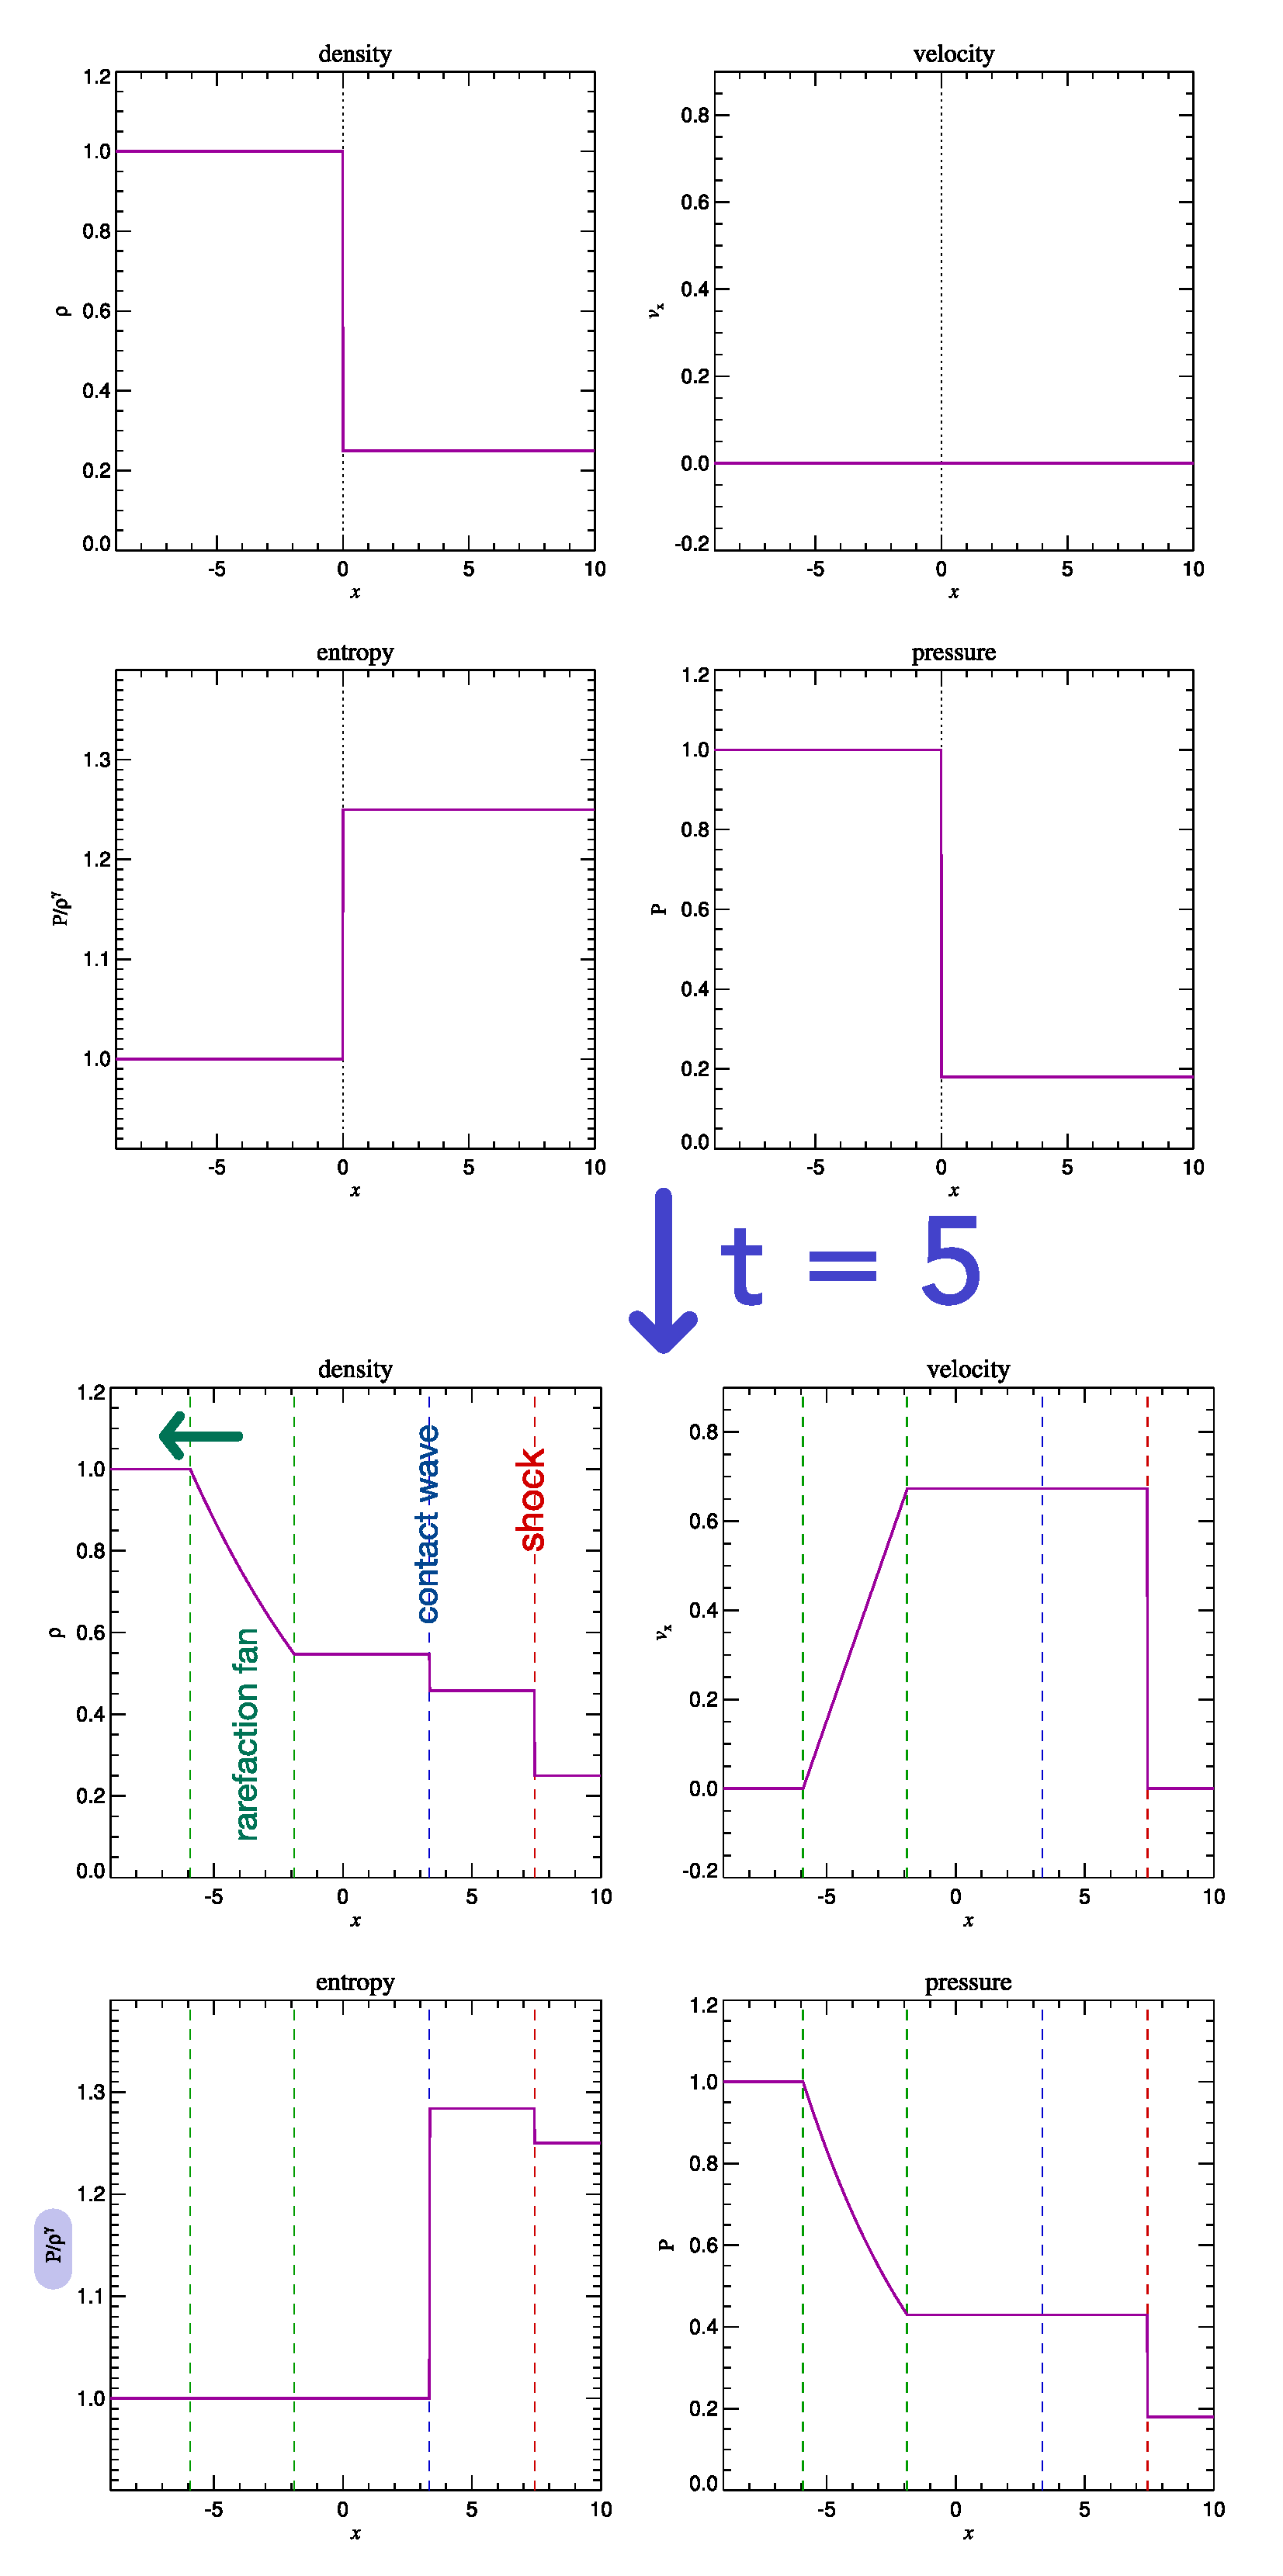
\includegraphics[width=0.6\textwidth]{figures/riemann_problem_example.pdf}
    \caption{Example Riemann-Problem situation}
    \label{fig:riemann_problem_example_s}
\end{figure}

\note{For an isentropic process $dS = 0$, the entropic function $A(s) = \frac{P}{\rho^\gamma} = \text{const.}$ so we can
use it as a proxy for entropy.}

\subsubsection*{Fluid instabilities}
Fluid instabilities are the rapid growth of small perturbations, tapping
into a source of free energy (if perturbations have a dispersion
relation with positive imaginary part). Consider two phases $(\rho_1,v_1)$ and
$(\rho_2,v_2)$ above each other.
\begin{itemize}
    \item Rayleigh-Taylor instability $v_1=v_2=0$ in $\vec{g}$-field: when the
    denser fluid is on-top, instability as of buoyancy
    \item Kelvin-Helmholtz instability $\vec{g} = 0$: sharp velocity gradients
    are unstable, eddies grow and break into turbulence
    \item Jeans-instability: in self-gravitating fluids, where denser regions can grow and collapse under their own attraction
\end{itemize}

\subsubsection*{Turbulent flow}
In contrast to laminar flow, turbulent flow is chaotic.

\paragraph*{How to quantify turbulence - Reynolds number} The Reynolds number is given by
\begin{equation}
    \begin{gathered}
        Re = \frac{\text{advective term}}{\text{frictional term}} = \frac{|(\vec{v}\cdot \vec{\nabla})\vec{v}|}{\nu \vec{\nabla}^2 \vec{v}} = \frac{V_0 L_0}{\nu} \\
        \text{with } V_0 = \text{characteristic velocity}, \quad L_0 = \text{characteristic length scale}, \\ \nu = \text{kinematic viscosity} = \frac{\eta}{\rho} \sim \lambda_{mfp} v_{th} \\
        \text{with } \lambda_{mfp} = \text{mean free path}, \quad v_{th} = \text{thermal velocity}
    \end{gathered}
\end{equation}
where turbulent flows have a high Reynolds number $Re > 3.5 \cdot 10^3$ (interstellar medium e.g. $Re \sim 10^8$, oceans ($\nu_\text{water} \sim 10^{-6} \m^2 \s^{-1}$) and
the atmosphere are also turbulent on the usual scales (except for boundary layers))
- the chaotic advective term generates turbulence faster than it can be dissipated. For
$Re \rightarrow \infty$ we obtain the Euler equations.

\paragraph*{Subsonic and supersonic turbulence}
\begin{itemize}
    \item subsonic (incompressible) turbulence: information speed higher than transport speed $\rightarrow$ assume $\vec{\nabla} \cdot \vec{v} = 0$, so in Fourier space $\vec{k} \cdot \vec{v} = 0$  $\rightarrow$ only source free, rotational turbulence
    \item supersonic turbulence, shocks $\mathcal{M} \gg 1$
    \begin{itemize}
        \item 1D: 1 compressive mode
        \item 2D: 1 compressive mode, 1 solenoidal mode
        \item 3D: 1 compressive mode, 2 solenoidal modes
    \end{itemize}
\end{itemize}

\paragraph*{Schematic concept of turbulence}
In 3D
\begin{itemize}
    \item \textbf{injection range} energy is injected on macroscopic scales, typical scale $L$, velocity $v$
    \item \textbf{inertial range} large eddies break up into smaller eddies and energy is transferred to smaller scales, vorticity ($\vec{\zeta} = \vec{\nabla}\times \vec{v}$) is conserved and no energy is dissipated,
    only from dimensional analysis (Kolmogorov theory) we can find that the smaller eddies have smaller velocity but higher
    vorticity and are less volume filling.
    \item \textbf{dissipation range} at the microscopic viscous scale ($\lambda_{visc}$, roughly the mean free path $\lambda_{mfp}$) energy is dissipated into viscous heat
\end{itemize}
In 2D the energy flow is reverted from small to large (inverse cascade). The
spectrum of turbulent kinetic energy over different eddy sizes (large
eddy $\rightarrow$ low wave number, small eddy $\rightarrow$ high wavenumber)
is illustrated in figure \ref{fig:kolmogorov_spectrum_s}.

\begin{figure}[!htb]
    \centering
    \includesvg[width=0.9\textwidth]{figures/kol_power.svg}
    \caption{Kolmogorov energy spectrum}
    \label{fig:kolmogorov_spectrum_s}
\end{figure}

\subsection*{Types of PDEs and numerical approaches for solving them}
We now consider equations with derivatives of dependent variables
with respect to not one (ODE) but possibly many independent variables
(PDE) e.g. place and time.

\paragraph*{Basic properties of PDEs}
\begin{itemize}
    \item \textcolor{blue1}{Order of the PDE:} Order of the highest occuring derivative
    \item \textcolor{blue1}{Linearity:} If the dependent variable and all its derivatives only occur linearly (no $\sqrt{\partial_x u}$), the PDE is linear and if $u_1$ and $u_2$ are solutions to the PDE, $c_1u_1+c_2u_2$ are as well (\textcolor{blue1}{superposition})
    \item \textcolor{blue1}{Homogeneity:} The PDE is homogeneous, if all terms contain the dependent variable or its derivatives, so if there is no source term
\end{itemize}

\paragraph*{Classification of 2nd order PDEs with one dependent and two independent variables}
The homogeneous solutions of PDEs 
\begin{equation}
    a \frac{\partial^2 u}{\partial x^2}+b \frac{\partial^2 u}{\partial x \partial y}+c \frac{\partial^2 u}{\partial y^2}+d \frac{\partial u}{\partial x}+e \frac{\partial u}{\partial y}+f u=g, \quad a, b, c \text { not all zero }
\end{equation}
are conic section in $k$-space, with classification

\begin{equation}
    \text { The PDE is }\left\{\begin{array}{c}
    \text { hyperbolic if } D>0 \\
    \text { parabolic if } D=0, \\
    \text { elliptic if } D<0
    \end{array} \quad \Delta=\left|\begin{array}{cc}
    a & b / 2 \\
    b / 2 & c
    \end{array}\right|, \quad D=-4 \Delta=b^2-4 a c\right.
\end{equation}

and \textbf{qualitative differences}

\begin{itemize}
    \item \textcolor{blue1}{Elliptic}
    \begin{itemize}
        \item often describe static problems (no time dependence)
        \item e.g. Poisson equation (here 2D): $(\partial_x^2 + \partial_x^2) \phi = 4\pi G \rho$.
    \end{itemize}
    \item \textcolor{blue1}{Parabolic}
    \begin{itemize}
        \item often of second order, describing slowly changing processes like diffusion, becoming smoother with time
        \item e.g. diffusion equation $\partial_t u = D \partial_x^2 u$.
    \end{itemize}
    \item \textcolor{blue1}{Hyperbolic}
    \begin{itemize}
        \item typically describe dynamical processes in physics; disturbances have finite propagation speed; solutions can develop steep regions and real discontinuities
        \item e.g. 1D wave equation $\partial_t^2 u - c_s^2 \partial_x^2 u = 0$.
        \item e.g. the advection equation $\partial_t u + v \partial_x u = 0$.
    \end{itemize}
\end{itemize}

\paragraph*{Hyperbolic first order homogeneous PDE systems}
The system
\begin{equation}
    \partial_t \vec{u} + \left(\mat{A} \mat{\nabla}_\vec{x} \right) \vec{u} = 0, \quad \mat{A} \text { with entries } A_{i j}, \quad \mat{\nabla}_\vec{x} = \text{diag}(\partial_{x_1}, \dots, \partial_{x_n})
\end{equation}
or analogously the conservation law
\begin{equation}
    \partial_t \vec{u} + \vec{\nabla}_\vec{x} \cdot \mat{F}(\vec{u}) = \partial_t \vec{u} + (\underbrace{\mat{\nabla}_\vec{u} \mat{F}(\vec{u})}_{:=\mat{A}}) \mat{\nabla}_\vec{x} \vec{u} = 0
\end{equation}
is hyperbolic if $\mat{A}$ is diagonalizable with real eigenvalues.
\note{The classification introduced has its limits: What type the Navier-Stokes equation
is seems different to tell, often \textit{hyperbolic} is used as \textit{advection-dominated} (the advection equation is hyperbolic) and \textit{parabolic} as \textit{diffusion-dominated} (the diffusion equation is parabolic) and then the Navier
stokes equation can be either depending on the Reynolds number.}

\paragraph*{Overview on PDE solvers}
\begin{itemize}
    \item \textcolor{blue1}{Finite difference methods:} Differential operators are approximated by finite difference operators, usually on a regular (Cartesian) mesh
    \item \textcolor{blue1}{Finite volume methods:} Useful for hyperbolic conservation 
    laws. We consider quantities averaged over finite volumes around mesh cells where 
    divergence terms in a PDE turn into fluxes through the cells surface ($\rightarrow$ conservative 
    method, fluxes are not lost). Exact expressions for the average value of the solution over some volumes 
    are calculated and from these averages solutions within the cells can be reconstructed. This \textbf{contrasts with 
    finite difference methods where derivatives are approximated based on nodal values and finite element 
    methods where local approximations are made using local data} and stitched together to a global solution.
    \item \textcolor{blue1}{Spectral methods:} The PDE is converted into an algebraic form (e.g. by Fourier transform), the solution is represented by a linear combination of functions (e.g. the plane waves from the inverse Fourier transform).
    \item \textcolor{blue1}{Method of lines:} All derivatives but one are approximated by finite differences, leading to an ODE system, where we can use ODE solvers. \textbf{Time-dependent problems:} Consider a time-dependent problem on a 1D grid, $x_i, i=1,...,N$. Each point yields and ODE for the time evolution of the solution at that point, dependent on e.g. the solution on neighboring points $\rightarrow$ $N$ coupled ODEs.
    \item \textcolor{blue1}{Finite element methods:} The simulation domain is divided into cells (elements, arbitrary shape, unstructured mesh) and the solution on each cell approximated in form of a simple (polynomial) function. The solutions from the cells are linearly combined and we solve for the coefficients, based on a weak
    formulation of our original problem (e.g. Galerkin weighting).
\end{itemize}

\textcolor{blue1}{Example for the method of lines: } Consider the 1D heat equation
\begin{equation}
    \partial_t u - \lambda^2 \partial_x^2 u = 0
\end{equation}
where discretizing the spatial derivative leaves us with an ODE in time.
\greenbox{\textbf{How to discretize the 2nd order derivative $\partial_x^2 u$?}: Second order Taylor expansion yields
\begin{equation}
    \begin{aligned}
        u(x+\Delta x) &= u(x) + \Delta x \partial_x u(x) + \frac{1}{2} \Delta x^2 \partial_x^2 u(x) + \mathcal{O}(\Delta x^3) \\
        u(x-\Delta x) &= u(x) - \Delta x \partial_x u(x) + \frac{1}{2} \Delta x^2 \partial_x^2 u(x) + \mathcal{O}(\Delta x^3)
    \end{aligned}
\end{equation}}

\subsection*{Simple finite difference advection solver - awareness for information flow}
Let us start with the simple advection equation
\begin{equation}
    \partial_t u + v \partial_x u = 0
\end{equation}
with known solution $u(x,t) = q(x - vt)$ for $u(x,t=0) = q(x)$.
\textcolor{red1}{The central difference explicit Euler combination}
\begin{equation}
    u_i^{(n+1)}=u_i^{(n)}-v \frac{u_{i+1}^{(n)}-u_{i-1}^{(n)}}{2 h} \Delta t
\end{equation}
\textcolor{red1}{fails miserably, because in the true system, information
only flows in the direction specified by $v$}. \textcolor{green1}{Directional
splitting minding the information flow yields}
\begin{equation}
    \begin{aligned}
        v > 0&: u_i^{(n+1)} = u_i^{(n)} - v \frac{u_i^{(n)} - u_{i-1}^{(n)}}{h} \Delta t  \\
        v < 0&: u_i^{(n+1)} = u_i^{(n)} - v \frac{u_{i+1}^{(n)} - u_{i}^{(n)}}{h} \Delta t 
    \end{aligned}
\end{equation}
\problem{We do not get perfect advection but a \textbf{numerically smoothed result}.
This can be seen by writing the upwind scheme as a central difference scheme plus 
diffusion term with $D = \frac{vh}{2}$, grid spacing $h$, so
\begin{itemize}
    \item numerical diffusion cannot be reduced by taking a smaller timestep
    \item for smaller grid-spacing, numerical diffusion can be reduced
\end{itemize}
}
\paragraph*{CFL criterion} As we only consider $u_{i-1}$ and not also $u_{i-2}$
in the upwind scheme
\begin{equation}
    \Delta t \leq \frac{h}{v}
\end{equation}
our scheme would need to incorparate information from also more distant neighbors
in the updates.

\paragraph*{More general advective setting} By writing $q_1 = \rho$, $q_2 = \rho v$,
the isothermal 1D Euler equation becomes
\begin{equation}
    \begin{gathered}
        \partial_t q_1 + \partial_x (q_1 v) = 0 \\
        \partial_t q_2 + \partial_x (q_2 v) = -c_s^2 \partial_x q_1
    \end{gathered}
\end{equation}
where for the advective updates of $q_1$ and $q_2$ the flux of information
is considered based on the intercell approximations
\begin{equation}
    v_{i+\frac{1}{2}} = \frac{1}{2} \cdot \left( \frac{q_{2,i}}{q_{1,i}} + \frac{q_{2,i+1}}{q_{1,i+1}} \right)
\end{equation}
(for the derivatives $\partial_x v$ and $-c_s^2 \partial_x q_1$ central differencing is fine).

\subsection*{Finite Volume Method and Approximate Riemann Solver}
\bluebox{In the following we present an Eulerian fluid solver, so we represent
the fluid by values of the bulk properties on cells at fixed positions in space.}
Consider the hyperbolic conservation law
\begin{equation}
    \partial_t \vec{U} + \partial_x \vec{F}(\vec{U}) = 0, \quad \text{e.g. for Euler-eq. in 1D: } \vec{U} = \begin{pmatrix}
        \rho \\
        \rho v \\
        \rho e
    \end{pmatrix}
\end{equation}
for now with a multidimensional state vector but only one spatial dimension.
\idea{Formulate a scheme based on cell averages
\begin{equation}
    \vec{U}_i = \frac{1}{V_i} \int_{\text{cell} i}{\vec{U}(\vec{x})} dV
\end{equation}
where cell values are updated based on intercell fluxes such that no
flux is lost, i.e. $\vec{U}$ over the whole domain is conserved.
}
\subsubsection*{1D Godunov scheme} Conservation of $\vec{U}$ is naturally captured in
\begin{equation}
    \Delta x \cdot \vec{U}_i^{(n+1)}= \Delta x \cdot \vec{U}_i^{(n)} + \Delta t \left[\underbrace{\vec{F}^*_{i-\frac{1}{2}}}_{\text{flux from left into cell}}-\underbrace{\vec{F}^*_{i+\frac{1}{2}}}_{\text{out on the right}}\right]
\end{equation}
so
\begin{equation}
    \vec{U}_i^{(n+1)}=\vec{U}_i^{(n)}+\frac{\Delta t}{\Delta x}\left[\vec{F}^*_{i-\frac{1}{2}}-\vec{F}^*_{i+\frac{1}{2}}\right]
\end{equation}
where the fluxes follow from solving Riemann problems at the boundaries.
\redbox{\begin{itemize}
    \item CFL needs to be obeyed so we have independent Riemann problems at the boundaries
    \item $\vec{U}$ is not piecewise constant in reality, so while $\vec{U}$ is conserved, the cell averages
    will deviate from the true averages
\end{itemize}}

\subsubsection*{Approximate HLL Riemann Solver to calculate the intercell flux}
Exact Riemann solver are often too costly, so we make simplifying assumptions.
\paragraph*{Problem statement} For the 1D conservation law
\begin{equation}
    \partial_t u(x) + \partial_x f(u) = 0
\end{equation}
with piecewise initial values
\begin{equation}
    u(x, t=0)=\left\{\begin{array}{l}
    u_L \text { for } x<0 \\
    u_R \text { for } x \geq 0
    \end{array}, \quad \text { cell interface at } x=0\right.
\end{equation}
and assuming the speed of the fastest moving wave to the left $S_L$ and
right $S_R$ to be given, we make the simplifying assumptions that
\begin{itemize}
    \item $\forall x \in [S_Lt,S_Rt]$ the middle state $u^{HLL} = u^*$ holds and is constant across the time step
    \item elsewhere, the previous states $u_L,u_R$ continue to hold, as shown in figure \ref{fig:char_hll_s}
\end{itemize}

\begin{figure}[htb!]
    \centering
    \includesvg[width=0.8\textwidth]{figures/hll2.svg}
    \caption{Characteristics of the Riemann problem and HLL approach.}
    \label{fig:char_hll_s}
\end{figure}

\paragraph*{Expression for $u^{HLL}$} Based on the simple balance equation
\begin{equation}
    \text{start state} \cdot \text{volume} + \text{net flux into volume} \cdot \Delta t = \text{end state} \cdot \text{volume}
\end{equation}
over $[\Delta t S_L,\Delta t S_R]$, so
\begin{equation}
    - \Delta t S_L u_L + \Delta t S_R u_R + (f_L - f_R) \cdot \Delta t = (- \Delta t S_L + \Delta t S_R) \cdot u^{HLL}
\end{equation}
we find
\begin{equation}
    u^{H L L}=\frac{S_R u_R-S_L u_L+f_L-f_R}{S_R-S_L}
\end{equation}

\paragraph*{Expression for the intercell flux $f^{HLL} = f^*$}
By the analogous balance equation in $x \in [S_L T,0]$ and $x \in [0,S_R T]$,
we find
\begin{equation}
    f^{H L L}=f_L+S_L\left(u^{H L L}-u_L\right)=f_R+S_R\left(u^{H L L}-u_R\right)
\end{equation}
\note{E.g. when both $S_L,S_R>0$, we would take $f_L$ as the intercell flux
to comply with the unidirectional information flow.}

\paragraph*{Flux for the Godunov scheme}
With these results, we get
\begin{equation}
    F_{i+\frac{1}{2}}^{H L L}=\frac{S_R^+ F_{i+1}-S_L^- F_i+S_L^- S_R^+\left(U_{i+1}-U_i\right)}{S_R^+-S_L^-}, \quad S_R^+ = \max(0, S_R), \quad S_L^- = \min(0, S_L)
\end{equation}

\paragraph*{What approach to use for the maximum wave velocities $S_L$ and $S_R$?}
An easy approach based on the bulk velocities $v_L,v_R$ and the respective speeds
of sound $a_L^2 = \gamma P_L \slash \rho_L$ and $a_L^2 = \gamma P_L \slash \rho_L$
is
\begin{equation}
    S_L = v_L - a_L, \quad S_R = v_R + a_R
\end{equation}

\subsubsection*{Extension of Godunov's scheme to higher dimensions}
\begin{itemize}
    \item dimensional splitting: Based on the 1D update scheme and the full fluid state
    vector, we can write the higher-dimensional update as a concatenation of 1D updates,
    e.g. \begin{equation}
        \vec{U}^{(n+1)}=x\left(\frac{\Delta t}{2}\right) \mathcal{Y}\left(\frac{\Delta t}{2}\right) \mathcal{Z}(\Delta t) \mathcal{Y}\left(\frac{\Delta t}{2}\right) \mathcal{X}\left(\frac{\Delta t}{2}\right) \vec{U}^{(n)}
    \end{equation}
    is 2nd order accurate.
    \item unsplit schemes: all fluxes ($3$ in $3$D) are calculated based on the same starting state
    and applied simultaneously
\end{itemize}

\subsubsection*{Extensions for higher accuracy}
\paragraph*{What is a scheme's order?} A schemes order is based on the scaling of 
the $L1$ error between true ($\rho(x)$) and approximated ($\rho_i$) solution.
\begin{equation}
    L1 = \frac{1}{N} \sum_{i=1}^{N}{\left| \rho_i - \rho(x_i) \right|} \propto \Delta x^\text{order}
\end{equation}
\greenbox{Doubling the resolution will quarter the error in a 2nd order accurate scheme.}

\paragraph*{Linear Reconstruction for 2nd order accuracy} While
we still only have one fluid state vector stored per cell, the fluxes 
are calculated based on a piece wise linear reconstruction on the cells
(reconstruct - evolve - average).

To be 2nd order accurate in time and space, we use a linear prediction
of the boundary values at $t + \Delta t \slash 2$ (\textbf{MUCSL-Hancock
scheme})
\begin{equation}
    \begin{gathered}
        \vec{U}_{i+\frac{1}{2}}^L=\vec{U}_i+\mathcolor{yellow1}{\left(\partial_x \vec{U}\right)_i} \frac{\Delta x}{2}+\mathcolor{blue1}{\left(\partial_t \vec{U}\right)_i} \frac{\Delta t}{2}, \quad \vec{U}_{i+\frac{1}{2}}^R=\vec{U}_{i+1}-\mathcolor{yellow1}{\left(\partial_x \vec{U}\right)_{i+1}}  \frac{\Delta x}{2}+ \mathcolor{blue1}{\left(\partial_t \vec{U}\right)_{i+1}} \frac{\Delta t}{2} \\
        \mathcolor{yellow1}{\left(\partial_x \vec{U}\right)_i \text{ calculated from finite difference approach + slope limiting}}
    \end{gathered}   
\end{equation}
where the derivative in time is estimated based on the
derivative in space using the conservation law
we are trying to solve (e.g. Euler eq.)
\begin{equation}
    \begin{gathered}
        \partial_t \vec{U} + \partial_x \vec{F}(\vec{U}) \underbrace{=}_{\text{quasi-linear form}} \partial_t \vec{U} + \mat{J}_\vec{U}(\vec{F})\cdot \partial_x \vec{U} = 0 \rightarrow \boxed{\partial_t \vec{U} = - \mat{J}_\vec{u}(\vec{F})\cdot \partial_x \vec{U}} \\
        \text{with Jacobian matrix } \mat{J}_\vec{U}(\vec{F}) \text{ of } \vec{F}(\vec{U}) \text{ with respect to } \vec{U}, \quad \left. \mat{J}_\vec{U}(\vec{F}) \right|_{\vec{U} = \vec{U}} =: \mat{A}(\vec{U})
    \end{gathered}
\end{equation}
One can go even higher order e.g. by piecewise parabolic reconstruction.
\greenbox{We get sharper, more accurate solutions with high order schemes,
while lower schemes smear solutions out.}
\problem{Higher order schemes are more expensive and create strong oscillations
at discontinuities (which lower order schemes do not). Linear numerical schemes
for solving PDEs having the property of not generating new extrema can at
most be first-order accurate (Godunov's theorem).}

\paragraph*{Flux limiters}\mbox{}\\
\idea{Non-linearly switch between fluxes, taking the low order where necessary and
high order where possible, which with the right flux limiter allows our scheme
to still be total variation diminishing.}
The flux limiter concept is illustrated in figure
\begin{figure}[htb!]
    \centering
    \includesvg[width=0.8\textwidth]{figures/flux_limiter.svg}
    \caption{Flux limiter concept.}
    \label{fig:flux_limiter_s}
\end{figure}

\subsection*{Smoothed Particle Hydrodynamics}
SPH is a mesh-free Lagrangian scheme where we discretize the fluid into SPH-particles
(not the real ones) with masses $m_i$ and size $\Delta r_i^3 \sim \frac{m_i}{\rho_i}$, 
surrounded by smoothing kernels and pushed forward
using the Lagrangian fluid equations.

\paragraph*{Kernelized Fluid Variable representation} The kernelized representation
of a fluid variable $F$ is given by
\begin{equation}
    F_s(\vec{r}_i) \equiv\langle F(\vec{r}_i)\rangle \simeq \sum_{j=1}^{N_i} \frac{m_j}{\rho_j} F_j W\left(\vec{r}_i-\vec{r}_j, h\right), \quad \text { number of neighbors } N_i
\end{equation}
which is differentiable everywhere and the spatial dependency has moved
into the kernel - nice for spatial derivatives. For the density
we get
\begin{equation}
    \rho_s (\vec{r}_i) = \sum_{j=1}^{N_i} m_j W(\vec{r}_i - \vec{r}_j,h)
\end{equation}
\paragraph*{Kernel and smoothing length} The kernel should have finite support
so that to calculate the value of a fluid quantity at a poin $\vec{r}_i$ only
the neighboring SPH-particles have to be considered.
\problem{There is no one-size fits all smoothing length - in rarefied
regions we want $h$ to be larger (so that the kernelized expression
still represents a fluid) and in denser regions smaller (to not smooth out
all the details.)}
The principal ways of making $h$ adaptive are
\begin{itemize}
    \item gather-approach: the smoothing length is chosen for each point of evaluation (total mass not exactly conserved)
    \item scatter-approach: each SPH-particle has its own smoothing length (total mass conserved)
\end{itemize}
where $h$ is chosen e.g. such that the mass in a $h^3$ ball remains constant or that
always the same number of neighbors is considered.
\note{For particles the different SPH-particles to see themselves on the same footing,
we have to symmetrize (to get antisymmetric forces later on)
\begin{equation}
    h_{ij} = \frac{h_i + h_j}{2}, \quad \text{or geometric mean} \quad h_{ij} = \sqrt{h_i h_j}
\end{equation}
}

\paragraph*{Forwarding the SPH-particles - simulation scheme} In the simplest
possible scheme, one only considers the pressure gradient force
\begin{equation}
    \vec{a}^{\text{pressure}} = -\frac{\vec{\nabla}P}{\rho}
\end{equation}
where a symmetrized SPH equation of motion can be followed as
\begin{equation}
    \vec{a}_i^{\text{pressure}} = -\sum_{j=1}^{N_i} m_j\left[\frac{P_j}{\rho_j^2}+\frac{P_i}{\rho_i^2}\right] \cdot \vec{\nabla}_i W_{i j}
\end{equation}
which is then used to forward the SPH-particles, e.g. using the Leapfrog method.
\begin{enumerate}
    \item In a first loop calculate all $\rho_i$ at the SPH-particles positions given their current positions
    \item In a second loop calculate the forces on the SPH-particles and forward them a timestep,
    obeying the CFL criterion (if the timestep is taken too long, we will forward
    the particles based on a density distribution that is not valid anymore), then go back to step $1$
\end{enumerate}
\note{Mind that $h$ depends on $\vec{r}_j$ as of the adaptive smoothing length, e.g.
by $\rho_j h_j^3 = \text{const.}$.
With this the above equation can also be yielded from a Lagrangian derivation, that
directly shows that linear and angular momentum as well as energy are conserved.
}

\paragraph*{Artificial viscosity}\mbox{}\\
\problem{The above SPH-scheme perfectly conserves the thermodynamic
specific entropy (not the entropy of our SPH-particles), so shocks -
in which entropy is generated and kinetic energy dissipated to head -
will never be resolved.}
\idea{Add artificial viscosity $\Pi_{ij}$ that is turned on if two particles
$i,j$ rapidly approach each other / come very close 
(also avoid interpenetration). To not add artificial viscosity to shear flow
turn the artificial viscosity down if vorticity (rotation of 
the velocity field) is high (shear flow balsara corresion).}
Including possibly gravity, the SPH momentum equation becomes
\begin{equation}
    \frac{d \vec{v}_i}{d t}=-\sum_{j=1}^{N_i} m_j\left(\frac{p_i}{\rho_i^2}+\frac{p_j}{\rho_j^2}+\Pi_{i j}\right) \vec{\nabla}_i W\left(r_{i j}, h_{i j}\right)-\vec{\nabla} \phi_i
\end{equation}

\paragraph*{Advantages and disadvantages of SPH} See table \ref{tab:advantages_disadvantages_sph_s}

\begin{table}[!htb]
    \centering
    \begin{tabular}{p{0.45\textwidth}|p{0.45\textwidth}}
        \textcolor{green1}{Advantages} & \textcolor{red1}{Disadvantages} \\
        \hline \\
        \begin{itemize}
            \item versatile and simple
            \item avoids numerical diffusion issues arising when advection is not aligned with the mesh
            \item automatically adaptive resolution, can cover large ranges in density and space
            \item excellent conservation properties (energy, linear and angular momentum, not guarantueed in Eulerian codes)
            \item inherent mass conservation
            \item Galilean invariant and free from advection errors
            \item can deal with complicated geometries as mesh-free
            \item simple and transparent codes
            \item very robust
            \item as a particle scheme it is good for describing the transition from gaseous to stellar dynamical systems (e.g. formation of stellar clusters)
        \end{itemize} &
        \begin{itemize}
            \item limited accuracy in multi-D flow
            \item The number of neighboring particles (based on the neighbors positions we calculate the density and then equations of motion at the particle of interest) in SPH is far greater than the number of neighboring nodes in mesh based methods
            \item low density regions are more poorly resolved
            \item poorly handles shocks
            \item noise as of discrete sums over limited neighbor set
            \item jitter develops
            \item fluid instabilities arcoss contact discontinuities are problematic such as Kelvin helmholtz instabilities
            \item artificial viscosity limits the Reynolds number which can be reached
            \item low convergence rate \tablefootnote{Convergence in the SPH case means that with increasing number of SPH particles we approach the correct fluid behavior.}
            \item approximation of boundary conditions can be difficult
            \item formation of voids
            \item free surfaces can be problematic (density underestimated there)
            \item magnetic fields are hard to handle (problems with stability and $\vec{\nabla} \cdot \vec{B} = 0$ requirement)
        \end{itemize} \\
    \end{tabular}
    \caption{Advantages and disadvantages of SPH.}
    \label{tab:advantages_disadvantages_sph_s}
\end{table}

\subsection*{Finite Element Methods}
\greenbox{\textbf{Idea of FEMs:} In FEMs the solution domain is structured into finite
elements with nodes on which base functions sit. The partial differential equation (or rather
a weak form\footnote{Weak here means, that the differential equation must not hold strictly locally,
but for instance an integrated residual is to be zero, not the residual everywhere itself.} of it)
turns into equations for the (finitely many) weights of those basis functions. \textcolor{green1}{Central advantage}:
we can use very complex geometries for the elements.}
\paragraph*{FEM for solving a linear PDE}
For the PDE
\begin{equation}
    L\phi + s = 0, \quad \text{ linear differential operator } L, \text{ source term } s, \text{ solution } \phi
\end{equation}
dependent on $x$ (here 1D but possibly many spatial coordinates),
we make the ansatz for the solution on the $k$-th element
\begin{equation}
    \begin{gathered}
        \phi^{(k)}(x) = \phi_1^{(k)} N_1^{(k)}(x) + \phi_2^{(k)} N_2^{(k)}(x) + \dots + \phi_n^{(k)} N_n^{(k)}(x) \\
        \text{shape functions } N_i^{(k)}, \text{ zero outside k-th element}
    \end{gathered}
\end{equation}
which does not exactly solve the PDE but yields a residuum
\begin{equation}
    \begin{gathered}
        L\phi + s = R^{(k)}(x; \phi_1, \dots, \phi_n) = L\left(\sum_{j=1}^n \phi_j N_j(x) \right) + s \underbrace{=}_{L \text{ linear}} \sum_{j=1}^n \phi_j L N_j(x) + s \\
        \text{supscript } k \text{ to indicate this is the residual over the k-th element}
    \end{gathered}
\end{equation}
which is to be minimized in some sense
\begin{itemize}
    \item Ritz method
    \begin{equation}
        \int_{\text{domain}}{R\left(x;\{\phi_i\}_{i=1}^\mathcal{N} \right)} \, dx = 0
    \end{equation}
    \item Weighted Residual method
    \begin{equation}
        \int_{\text{domain}} {w_i(x) R\left(x;\{\phi_i\}_{i=1}^\mathcal{N} \right)} \, dx = 0, \quad i = 1,\dots,\mathcal{N}
    \end{equation}
    \begin{itemize}
        \item \textcolor{blue1}{Galerkin method}: Choose basis functions themselves as weights, so $w_i(x) = N_i(x)$, so
        \begin{equation}
            \int_{\text{domain}} N_i(x) R\left(x;\{\phi_i\}_{i=1}^\mathcal{N} \right) \, dx = 0, \quad i = 1,\dots,\mathcal{N}
        \end{equation}
        \textbf{from which a linear equation on the coefficients follows} as the linear
        operator only acts on the shape function $N_i$ as they capture the spatial dependence.
    \end{itemize}
\end{itemize}

\paragraph*{Discontinuous Galerkin Method for solving the Euler equations} To be able
to resolve shocks, we allow the solutions on the elements to be discontinous across
elements.
\begin{itemize}
    \item we \textbf{represent} the fluid one the cell by a sum of orthogonal polynomials capturing statial dependency (e.g. Legendre polynomials), weighted by time-dependent weights>
    \begin{equation}
        \begin{gathered}
            \vec{u}^{\mathcolor{yellow1}{(K)}}(\vec{x}, t)=\sum_{l=1}^{N(\mathcolor{green1}{k})} \vec{\omega}_l^{\mathcolor{yellow1}{(K)}}(t) \phi_l^{\mathcolor{yellow1}{(K)}}(\vec{x}) \\
            \text{element index } K, \quad \text{highest order polynomial degree } k
        \end{gathered}
    \end{equation}
    \note{The notation has changed, $\phi_l$ are the Legendre base functions.}
    \item the \textbf{initial weigths} are determined using the orthogonality of the polynomials by
        \begin{equation}
            \begin{aligned}
                \vec{\omega}_j^K(t)&=\frac{1}{|K|} \int_K \vec{u}^{(K)} \phi_j^{(K)} d V, \quad j=1, \ldots, N(k) \\
                                   \underset{\text{cubic cells}}&= \frac{1}{8} \int_{[-1,1]^3} \vec{u}^{(K)}(\vec{\xi}, t) \phi_j^{(K)}(\vec{\xi}) d^3 \vec{\xi} \\
                                                                \underset{\text{Gauss quad.}}&\approx \frac{1}{8} \sum_{q=1}^{(k+1)^3} \vec{u}^{(K)}\left(\vec{\xi}_q^{3 D}, t\right) \phi_j^{(K)}\left(\xi_q^{3 D}\right) w_q^{3 D}
            \end{aligned}
        \end{equation}
    with quadrature nodes $\vec{\xi}_q^{3 D}$ (Legendre polynomial roots) and quadrature weights $w_q^{3 D}$.
    \item the \textbf{weights are updated} based on the relaxed Galerking formulation of the Euler equations
    \begin{equation}
        \int_K\left[\partial_t \vec{u}^{(K)}+\sum_{\alpha=1}^3 \partial_{x_\alpha} f_\alpha\right] \phi_j^{(K)} d V=0
    \end{equation}
    so (integrate by parts and Gauss theorem)
    \begin{equation}
        \begin{gathered}
            \frac{d}{d t} \underbrace{\int_K \vec{u}^{(K)} \phi_j^K d V}_{\vec{w}_j^{(K)} \cdot |K|} + \sum_{\alpha=1}^3 \explain{\int_{\partial K} f_\alpha n_\alpha \phi_j^K d S}{evaluate using Gauss-Quad, unknown flux across discont. via Riemann solver} - \sum_{\alpha=1}^3 \explain{\int_K \vec{f}_\alpha \frac{\partial \phi_j^K}{\partial x_\alpha} d V}{evaluate via Gauss-Quad., interior flux known from state variable approx.} = 0 \\
            \text{normal vector } \vec{n} = \left( \begin{array}{c} n_1 \\ n_2 \\ n_3 \end{array} \right) \text{ on } \partial K
        \end{gathered}
    \end{equation}
    \item \textbf{increasing accuracy:} $p$-refinement is using a polynomial basis to higher orders on each element, $h$-refinement is using
    a finer grid where $p$-refinement is often advantageous.
\end{itemize}

\subsection*{Diffusion}
\subsubsection*{Derivation of the Diffusion Equation}
\paragraph*{Diffusion as a random Walk} Diffusion can be seen as a random
walk with step size $\lambda_{mfp} = \frac{1}{\sqrt{2}n\sigma}$ and number
of steps $N = \frac{t}{t_\text{rel}}$
with $t_{rel} = \frac{\lambda_{mfp}}{v}$ with 
$v:= \sqrt{\langle \vec{v}^2 \rangle}$ based on the equipartition 
theorem $\langle \frac{1}{2} m \vec{v}^2 \rangle = \frac{3}{2} k_B T$. Density
naturally spreads probabalisticly.
The additive distance from the origin based on many steps
is normally distributed as of the central limit theorem, with
\begin{equation}
    \langle x \rangle = 0, \quad \langle x^2 \rangle = N \sigma_s^2 = \frac{\lambda_{mfp}^2}{t_{rel}} t \rightarrow \boxed{\sqrt{\langle x^2 \rangle} \propto \sqrt{t}}
\end{equation}
\greenbox{\textbf{Central Limit Theorem:} Let $w(s) ds$ be the probability
of taking a step with length between $s$ and $s+ds$ with mean
$\langle s \rangle$ and variance $\sigma_s^2$. We make $N$ steps,
so the final position along one dimension is
\begin{equation}
    x = s_1 + s_2 + s_3 + \dots + s_N
\end{equation}
By the rules of the mean and variance, one finds
\begin{equation}
    \begin{gathered}
        \langle x \rangle = N \langle s \rangle, \quad \langle s \rangle = \int_{-\infty}^{\infty} s \cdot w(s) \, ds \\
        (\Delta x)^2 = \sigma_x^2 = \langle (x - \langle x \rangle)^2 \rangle = N \sigma_s^2
    \end{gathered}
\end{equation}
And the \textbf{Central Limit Theorem} states
\begin{equation}
    \label{eq:central_limit_theorem}
    \boxed{P(x) = \frac{1}{\sqrt{2\pi}\Delta x} \exp{\left( -\frac{(x-\langle x \rangle)^2}{2(\Delta x)^2} \right)}}
\end{equation}
if the moments $\langle s^n \rangle = \int_{-\infty}^{\infty} s^n w(s) \, ds$ are finite. The basis reasoning
is that one can show that for added random variables their sum converges to one distribution, and as added random
variables are distributed according to the convolution of their distributions and the convolution of two Gaussians is
a Gaussian, the sum of many random variables is a Gaussian.}
\paragraph*{Diffusion equation}
Based on Taylor expansion of (LHS in time, RHS in space)
\begin{equation}
    n(x,t+\Delta t) = \langle n(x-\Delta x,t) \rangle_{\Delta x \sim p(\cdot,\Delta t)}
\end{equation}
neglecting terms starting from $4$th order one finds
the \textbf{diffusion equation}
\begin{equation}
    \partial_t n(x,t) = \mathcolor{blue1}{\frac{\Delta x^2}{2 \Delta t}} \partial_x^2 n(x,t) = \mathcolor{blue1}{D} \partial_X^2 n(x,t)
\end{equation}
with
\begin{equation}
    \mathcolor{blue1}{\text{diffusion coefficient } D = \frac{\Delta x^2}{2 \Delta t} \propto \frac{\lambda_{mfp}^2}{t_{rel}}}
\end{equation}
The analytical solution can be found via Fourier transform.
\problem{An initial delta peak in the density evolves as a Gaussian which
implies infinite information speed - a result from our truncated expansion.}
\subsubsection*{Numerical solutions to the diffusion equation}
Consider $\partial_t u = D \partial_x^2 u$ and in the discretization write $u_{\text{space}}^{\text{(time)}}$.
\paragraph*{Simple but problematic central in space forward in time scheme}
\begin{equation}
    u_i^{(j+1)} = u_i^{(j)} + \alpha \left( u_{i+1}^{(j)} - 2 u_i^{(j)} + u_{i-1}^{(j)} \right), \quad \alpha = \frac{D \Delta t}{\Delta x^2}
\end{equation}
\problem{Based on how the density spreads with $\Delta x = \sqrt{2 D \Delta t}$, we get the
CFL criterion
\begin{equation}
    \alpha \leq \frac{1}{2} \leftrightarrow \Delta t \leq \frac{1}{2} \frac{\Delta x^2}{D}
\end{equation}
so if we want to double the resolution, we must quadruple the resolution in time (so in 3D: $\times 32$ cost).
}
\paragraph*{Implicit schemes to the help: Backward in time, central in space}
By evaluating the spatial derivative at $j+1$ (implicit), we get the linear system
\begin{equation}
    -\alpha u_{i+1}^{(j+1)} + (1+2\alpha) u_i^{(j+1)} - \alpha u_{i-1}^{(j+1)} = u_i^{(j)}
\end{equation}
\problem{This is unconditionally stable but only first order in time $\mathcal{O}(\Delta x^2, \Delta t)$.}

\paragraph*{Crank-Nicolson method} Here the spatial derivative is
evaluated at $j+\frac{1}{2}$ as the average of $j$ and $j+1$.
\begin{equation}
    \frac{u_i^{(j+1)}-u_i^{(j)}}{\Delta t}=D \frac{u_{i+1}^{\left(j+\frac{1}{2}\right)}-2 u_i^{\left(j+\frac{1}{2}\right)}+u_{i-1}^{\left(j+\frac{1}{2}\right)}}{\Delta x^2}, \quad \text { use avg. } u_i^{\left(j+\frac{1}{2}\right)}=\frac{u_i^{(j+1)}+u_i^{(j)}}{2}
\end{equation}
\greenbox{Advantage of Crank-Nicolson: $\mathcal{O}( \Delta x^2, \Delta t^2)$ (2nd order in space and time) and unconditionally stable.}

\subsubsection*{Flux limited diffusion}
To avoid the infinitely large signal speeds, we limit the diffusion flux by hand
based on
\begin{equation}
    \partial_t u = - \partial_x J, \quad J = - D \partial_x u, \quad \text{ansatz } J(x,t) = u(x,t) \cdot v, \quad \text{characteristic velocity } v
\end{equation}
where $v=-\frac{D \partial_x u}{u}$ is replaced by $\tilde{v}$ inspired by special relativity
$mv = \gamma(\tilde{v})m\tilde{v}$.

\subsection*{Solving Linear Equations with Iterative Solvers and the
Multigrid Technique}
\subsubsection*{Why do we need iterative methods?}
Linear systems we want to solve might be the linear system occuring
in multidimensional Newton-Raphson or e.g. in solving
the \textbf{discretized Poisson problem}
\begin{equation}
    \begin{gathered}
        \partial_x^2 \phi = 4\pi G \rho \rightarrow (\partial_x^2\phi) \approxeq \frac{\phi_{i+1} - 2\phi_i + \phi_{i-1}}{h^2}  \approxeq  4\pi G \rho_i \\
        i = 1,\dots,N, \quad \text{spacing } h
    \end{gathered}
\end{equation}
We write this as a matrix equation
\begin{equation}
    \mat{A} \vec{\phi} = \vec{b}, \quad \vec{\phi} = \left( \begin{array}{c} \phi_1 \\ \phi_2 \\ \vdots \\ \phi_N \end{array} \right), \quad \vec{b} = 4\pi G \vec{\rho}, \vec{\rho} = \left( \begin{array}{c} \rho_1 \\ \rho_2 \\ \vdots \\ \rho_N \end{array} \right)
\end{equation}
with in the case of periodic boundary conditions
\begin{equation}
    \mat{A} = \frac{1}{h^2} \left( \begin{array}{cccccc}
            -2 & 1 & 0 & \dots & 0 & 1 \\
            1 & -2 & 1 & 0 & \dots &  \\
            0 & 1 & -2 & 1 & 0 & \dots \\
            0 & 0 & \ddots & \ddots & \ddots & 0 \\
            0 & \dots &  & 1 & -2 & 1 \\
            1 & 0 & 0 & \dots & 1 & -2
        \end{array} \right)
\end{equation}

\redbox{\textbf{Why shouldn't we explicitly invert $\mat{A}$?}: 
While there are stable and fast (approximate) algorithms for
efficiently inverting $\mat{A}$ (e.g. the Monte Carlo approach \cite{mat_inv}), 
the inverse of a sparse matrix is dense in general.}

\problem{LU (or QU) decomposition are $\mathcal{O}(N^3)$ in the decomposition $\mat{A} = \mat{L}\mat{U}$
(but solutions to different $\vec{b}$ can then be obtained in $\mathcal{O}(N^2)$).}

\greenbox{\textbf{Special case of tridiagonal matrices}: Here the system of equations
can just be solved by top-down eliminating the lower diagonal and then bottom up
solving the system $\mathcal{O}(N)$.}

\subsubsection*{Jacobi iteration | simple but slow}
Based on the trivial split
\begin{equation}
    \begin{gathered}
        \mat{A} = \mat{D} - (\mat{L} + \mat{U}), \quad \text{diagonal part } \mat{D}, \quad \text{negative left-below-diagonal part} \mat{L} \\
        \text{negative right-above-diagonal part} \mat{U}
    \end{gathered}
\end{equation}
one obtains the fixed-point iteration
\begin{equation}
    \vec{x}^{(n+1)} = \mat{D}^{-1} \vec{b} + \mat{D}^{-1} (\mat{L} + \mat{U}) \vec{x}^{(n)}, \quad (\mat{D}^{-1})_{ii} = \frac{1}{A_{ii}}
\end{equation}
which converges if 
\begin{equation}
    \text{spectral radius } \rho_s(\mat{M}) \equiv \max_i{|\lambda_i|} < 1, \quad \mat{M} := \mat{D}^{-1} (\mat{L} + \mat{U})
\end{equation}
following from $\vec{e}^{(n+1)} = \vec{x}_{\text{exact}} - \vec{x}^{(n+1)} = \mat{M} \vec{e}^{(n)}$.

\subsubsection*{Gauss-Seidel iteration | faster but hard to parallelize}
\idea{Each Jacobi step consists of $N$ scalar updates, use the results from
previous scalar updates to get up to $2\times$ convervence speed (which is guaranteed
is $\mat{A}$ strictly diagonally dominant or symmetric and positive definite).}
\begin{equation}
    \vec{x}^{(n+1)} = \mat{D}^{-1} \mat{L} \vec{x}^{(n+1)} + \mat{D}^{-1} \mat{U} \vec{x}^{(n)} + \mat{D}^{-1} \vec{b}
\end{equation}
which is explicit as $\mat{L}$ is lower diagonal.
\problem{Hard to parallelize, as we have sequential dependence.}
\greenbox{\textbf{Avoiding sequential dependence - Red-black ordering:} If possible
split the $N$ updates into two groups where all updates within a group are
independent but the updates of the 2nd group depend on the ones from the first.}

\subsubsection*{Problem of longwave errors in Jacobi- and Gauss-Seidel}
While the stencil for the 2nd derivative only considers nearest neighbors (we have
a local constraint), we need to find a global solution to the potential such that
\begin{equation}
    \frac{\phi_{i+1} - 2\phi_i + \phi_{i-1}}{h^2}  \approxeq  4\pi G \rho_i
\end{equation}
holds everywhere.
\problem{In our iterative schemes information travels only one stencil at a time -
short wavelength errors (in (the Fourier transform of)
$\vec{e}^{(n)} = \vec{x}_{\text{exact}} - \vec{x}^{(n)}$) die out quickly, but
long wavelength errors take lots of iterations to decrease.}

\subsubsection*{Multigrid technique | longwave error correction}
Consider e.g. the setting of the Poisson problem. If
we take a coarse grid for our domain of interest, we will
quickly converge to the coarse solution (only by nearest neighbor
communication information quickly travels the whole domain), but we
want a detailed solution on a fine grid.
\greenbox{\textbf{Idea - Coarse grid error correction:} Consider
we start with a guess $\vec{\tilde{x}}^{(h)}$ on the fine grid with spacing $h$. Given
the easy-to-calculate residual
\begin{equation}
    \vec{r}^{(h)} = \vec{b} - \mat{A}\vec{\tilde{x}}^{(h)}
\end{equation}
the error
\begin{equation}
    \vec{e}^{(h)} = \vec{x}_\text{exact} - \vec{\tilde{x}}^{(h)} \quad \rightarrow \quad \vec{x}_\text{exact} = \vec{\tilde{x}}^{(h)} + \vec{e}^{(h)} 
\end{equation}
fullfills the linear equation
\begin{equation}
    \mat{A} \vec{x}_{\text{exact}} = \vec{b} \quad \rightarrow \quad \mat{A} (\vec{\tilde{x}}^{(h)} + \vec{e}^{(h)}) = \vec{b} \quad \rightarrow \quad \mat{A} \vec{e}^{(h)} = \vec{r}^{(h)}
\end{equation}
\textbf{So what if we could solve for the longwave error on the coarse grid
on by prolongation make a correction on the fine grid?}
}
\paragraph*{How to prolong and restrict (in 1D)?} We use the mapping
\begin{equation}
    \mat{I}_{\text{from this spacing}}^{\text{to this spacing}} \vec{x}^{(\text{from this spacing})} = \vec{x}^{(\text{to this spacing})}
\end{equation}
with the operations performed being $h \leftrightarrows 2h$ (so always
halving or doubling the grid point spacing) where by design
\begin{equation}
    \mat{I}_h^{2h} = c[\mat{I}_{2h}^{h}]^T
\end{equation}
(often problematic at edges), e.g.
\begin{equation}
    \begin{gathered}
        \text{prolongation: } \mat{I}_{2h}^{h} = \frac{1}{2}\left(\begin{array}{lll}
            1 & & \\
            2 & & \\
            1 & 1 & \\
            & 2 & \\
            & 1 & 1 \\
            & & 2 \\
            & & 1
            \end{array}\right) \\ \text{restriction: } \mat{I}_{h}^{2h} = \frac{1}{2} \left( \mat{I}_{2h}^{h} \right)^T = \frac{1}{4} \left(\begin{array}{lllllll}
                1 & 2 & 1 & & & & \\
                & & 1 & 2 & 1 & & \\
                & & & & 1 & 2 & 1
                \end{array}\right)
    \end{gathered}
\end{equation}
Short-hand notations can be found in table \ref{tab:pro_res_short_s}.

\begin{table}[H]
    \centering
    \begin{tabular}{|p{0.45\textwidth}|p{0.45\textwidth}|}
        \hline
        \textbf{Prolongation} & \textbf{Restriction} \\
        \hline
        We can write prolongation as
        \begin{equation}
            \text{1D prolongation: } \mat{I}_{2h}^{h}: \left] \begin{array}{lll} \frac{1}{2} & 1 & \frac{1}{2} \end{array} \right[
        \end{equation}
        meaning that every coarse point is added to three fine points with these respective weights (see previous example). &
        We can write restriction as
        \begin{equation}
            \text{1D restriction: } \mat{I}_{h}^{2h}: \left[ \begin{array}{lll} \frac{1}{4} & \frac{1}{2} & \frac{1}{4} \end{array} \right]
        \end{equation}
        - the coarse point is the weighted sum of the three fine points. \\
        \hline
    \end{tabular}
    \caption{Short-hand notations for prolongation and restriction.}
    \label{tab:pro_res_short_s}
\end{table}

\paragraph*{V-cycle}
Let us start with a (fine-grid) guess $\vec{\tilde{x}}^{(h)}$ for the problem
\begin{equation}
    \mat{A}^{(h)} \vec{x}^{(h)} = \vec{b}^{(h)}
\end{equation}
and we want to obtain an improvement $\vec{\tilde{x}'}^{(h)} = CG(\vec{\tilde{x}}^{(h)}, \vec{b}^{(h)})$.

$CG$ consists of the following steps
\begin{enumerate}
    \item Perform \textcolor{blue1}{one iterative \textit{relaxation}} step on the current grid $h$, e.g. Jacobi or Gauss-Seidel
    \item \textcolor{blue1}{Compute the residual}
    \begin{equation}
        \vec{r}^{(h)} = \vec{b} - \mat{A}\vec{\tilde{x}}^{(h)}
    \end{equation}
    \item \textcolor{blue1}{Restrict the residual} to the coarser mesh
    \begin{equation}
        \vec{r}^{(2h)} = \mat{I}_{h}^{2h}\vec{r}^{(h)}
    \end{equation}
    \item \textcolor{blue1}{Solve for the error on the coarser mesh}
    \begin{equation}
        \mat{A}^{(2h)}\vec{e}^{(2h)} = \vec{r}^{(2h)}, \quad \text{starting guess } \vec{\tilde{e}}^{(2h)} = \vec{0}
    \end{equation}
    \item \textcolor{blue1}{Correct $\vec{\tilde{x}}^{(h)}$ on the finer mesh} using the prolonged error
    $\vec{e}^{(h)} = \mat{I}_{2h}^{h} \vec{e}^{2h}$
    \begin{equation}
        \vec{\tilde{x}'}^{(h)} = \vec{\tilde{x}}^{(h)} + \vec{e}^{(h)}
    \end{equation}
    \item \textcolor{blue1}{Further iterative \textit{relaxation}} step on the fine mesh
\end{enumerate}

\bluebox{\textbf{How to solve for the error on the coarse mesh?: } Step 4 can be performed by 
recursively calling $CG(\vec{\tilde{x}}^{(2^ih)}, \vec{b}^{(2^ih)}), i\geq 1$ until 
a coarseness is reached where one can easily exactly solve or solve by multiple relaxation
steps.}

\bluebox{\textbf{How to find $\mat{A}^{(2h)}$ on the coarse mesh?: } Generally
in the \textbf{Galerkin coarse grid approximation} one defines
\begin{equation}
    \mat{A}^{(2h)} = \mat{I}_h^{2h} \mat{A}^{(h)} \mat{I}_{2h}^{h}
\end{equation}
which is an \textcolor{red1}{additional matrix operation that might enlarge the stencil (and so the computational cost), 
depending on the interpolation operator}. 

When $\mat{A}$ was brought forth by formulating a discretization in matrix form, we can
use the same discrete equations as one the fine grid (\textbf{direct method}). In other words, the same
stencil (\textit{Schablone}) is used to go over the points and collect for the linear relations,
e.g. for the 2D-Poisson - no matter the coarseness - we would construct $\mat{A}$ based on eq. \ref{eq:2dpoisson_disc}.}

The 6-step iteration process with a recursion call in step 4 leads to a cycle as
illustrated in figure \ref{fig:vcycle_s}.

\begin{figure}[H]
    \centering
    \includesvg[width=0.9\textwidth]{figures/vcycle2.svg}
    \caption{V-cycle.}
    \label{fig:vcycle_s}
\end{figure}

The V-cycle for the Poisson equation has the same cost as FFT-based methods but
requires less thread communication when parallelized.

\bluebox{\textbf{Computational costs}
\begin{equation}
    \begin{gathered}
        \text{computational cost per V-cycle:} \mathcal{O}(N_{\text{fine}}) \\
        \text{computational cost until convergence to machine error (mult. cycles) } \mathcal{O}(N_{\text{fine}} \log{N_{\text{fine}}}) \\
        \text{with } N_{\text{fine}} \text{ being the number of grid-cells on the fine grid} \\
    \end{gathered}
\end{equation}
}

\paragraph*{Full multigrid method} Here an initial guess is constructed
based on the true solution on the coarsest level which is prolonged
to the next-finer level, improved by a v-cycle, prolonged up again\dots
The cost is the same as for the V-cycle, dominated by $N_\text{fine}$.

\subsubsection*{Krylow subspace methods}
\paragraph*{Motivation} In numerical root-finding, the Jacobian can become too large
to be stored explicitly, but Jacobian vector products can easily
be calculated by forward AD. What if there was a linear solver
only depending on JVPs (generally matrix vector products)?

\paragraph*{Solving a linear system by minimizing the quadratic form}
Consider $\mat{A} \in \mathbb{R}^{N \times N}$ symmetric ($\mat{A}^T = \mat{A}$) and positive definite, so $\vec{x}^T \mat{A} \vec{x} > 0 \forall \vec{x}\in \mathbb{K}^N \setminus \{\vec{0}\}$ (only positive eigenvalues).
Then the following holds
\begin{equation}
    \mat{A}\vec{x} = \vec{b} \leftrightarrow \text{quadratic form } f(x) := \frac{1}{2} \vec{x}^T \mat{A} \vec{x} - \vec{x}^T \vec{b} \text{ is minimal}
\end{equation}
\problem{Steepest descent often takes steps in directions already taken. Steepest descent is good if our
parabolic quadratic form $f$ is nearly circular but the more elliptic $f$ is, the more problematic
steepest descent becomes.}

\paragraph*{Conjugate gradient method} By taking steps with 
residuals $\vec{r}^{(n)} = \vec{b} - \mat{A}\vec{x}^{(n)}$ orthogonal to $\mathcal{K}_n$
where $\mathcal{K}_n$ is the Krylow subspace
\begin{equation}
    \mathcal{K}_r := \mathcal{K}_r(\mat{A},\vec{b}) = \text{span} {(\vec{b}, \mat{A}\vec{b}, \mat{A}^2\vec{b}, \dots, \mat{A}^{r-1}\vec{b})}
\end{equation}
constructed with an orthogonal basis so that $\vec{r}^{(n)}$ is proportional
to the $n+1$th basis vector \textbf{we reach the true solution in at most $N$ steps}.
The directions taken are hereby conjugate ($\left(\vec{p}^{(j)} \right)^T \mat{A} \vec{p}^{(j)} = 0$ for $i \ne j$).

\subsection*{Fourier methods}
\subsubsection*{Motivation: The solution to Poisson's equation is 
a convolution in real space becoming a multiplication in Fourier space}
The analytical solution of Poissons equation
\begin{equation}
    \vec{\nabla}^2 \phi = 4\pi G \rho
\end{equation}
for the potential based on a mass density distribution
\begin{equation}
    \begin{gathered}
        \phi(\vec{x})=-G \int \frac{\rho\left(\vec{x}^{\prime}\right)}{\left|\vec{x}-\vec{x}^{\prime}\right|} d \vec{x}^{\prime}=\int g\left(\vec{x}-\vec{x}^{\prime}\right) \rho\left(\vec{x}^{\prime}\right) d \vec{x}^{\prime}=g \star \rho \\
        \text{Greens function of gravity } g(\vec{x}) = -\frac{G}{|\vec{x}|}
    \end{gathered}
\end{equation}
is a \textbf{convolution of the density with the Green's function of the Poisson equation}.

\greenbox{\textbf{Fast potential calculation by the Convolution theorem and FFT:} The 
Fourier transform of the convolution of two functions is equal to the product
of the individual Fourier transforms of those functions (\textbf{convolution theorem})
\begin{equation}
    \mathcal{F}(f \star g)=\mathcal{F}(f) \cdot \mathcal{F}(g), \quad \text { functions } f, g, \quad \text { Fourier transform } \mathcal{F}
\end{equation}
so for the Poisson problem
\begin{equation}
    \phi=\mathcal{F}^{-1}[\mathcal{F}(g) \cdot \mathcal{F}(\rho)], \quad \text { in Fourier space } \mathcal{F}(\phi)=: \hat{\phi}(\vec{k})=\hat{g}(\vec{k}) \cdot \hat{\rho}(\vec{k})
\end{equation}
with the Greens function in Fourier space being
\begin{equation}
    \hat{\phi}(\vec{k}) = -\frac{4\pi G}{\vec{k}^2} \hat{\rho}_\vec{k} \quad \rightarrow \quad \hat{g}(\vec{k}) = -\frac{4\pi G}{\vec{k}^2} 
\end{equation}
where for a density distribution given by discrete values (assuming periodic boundaries or use zero-padding)
$\{ \rho_i \}_{i=1}^N$, we can get $\{ \phi_i \}_{i=1}^N$ based on
\begin{enumerate}
    \item calculate $\{\hat{\rho}_{\vec{k}_i}\}_{i=1}^N$ in Fourier space by FFT in $\mathcal{O}(N\log N)$
    \item multiply $\{ \hat{\phi}_{\vec{k}_i} \}_{i=1}^N = \{\hat{\rho}_{\vec{k}_i}\cdot \hat{g}_{\vec{k}_i}\}_{i=1}^N$ in $\mathcal{O}(N)$
    \item get to $\{ \phi_i \}_{i=1}^N$ by FFT in $\mathcal{O}(N\log N)$
\end{enumerate}
which in total is $\mathcal{O}(N\log N)$.
}

\subsubsection*{Periodic and discrete Fourier transform (DFT)}
\begin{itemize}
    \item for a box with sidelength $L$ with smooth periodic boundaries, all possible
    modes are multiples of $\frac{2\pi}{L}$ (but we may need infinitely many modes)
    \item for discretized space $\vec{x} = \frac{L}{N}\vec{p}$, $p_1,p_2,p_3 \in \{ 0,1,\dots,N-1\}$
    finitely many modes ($N$ per dimension) are sufficient to accurately describe the distribution -
    all higher frequencies are aliased to lower ones
\end{itemize}
\begin{equation}
    \begin{gathered}
    \text { Fourier space } \hat{\rho}_{\vec{l}}=\frac{1}{N^3} \sum_{\vec{p}} \rho_{\vec{p}} \exp \left(-i \frac{2 \pi}{N} \vec{l} \cdot \vec{p}\right) \\
    \text { Real space } \rho_{\vec{p}}=\sum_{\vec{l}} \hat{\rho}_{\vec{l}} \exp \left(i \frac{2 \pi}{N} \vec{l} \cdot \vec{p}\right) \\
    \vec{l}\in\left(\begin{array}{l}
        \left\{-\frac{N}{2}, \ldots,-1,0,1, \ldots, \frac{N}{2}-1\right\} \\
        \left\{-\frac{N}{2}, \ldots,-1,0,1, \ldots, \frac{N}{2}-1\right\} \\
        \left\{-\frac{N}{2}, \ldots,-1,0,1, \ldots, \frac{N}{2}-1\right\}
    \end{array}\right), \quad \vec{p} \in \left(\begin{array}{l}
        \{0,1, \ldots, N-1\} \\
        \{0,1, \ldots, N-1\} \\
        \{0,1, \ldots, N-1\}
        \end{array}\right)
    \end{gathered}
\end{equation}
where
\begin{itemize}
    \item the centering in $\vec{k}$-space is by convention
    \item a shift of $\frac{2\pi N}{L}$ in $\vec{k}$ (so $N$ in an entry of $l$) will be aliased to the same mode, higher frequencies than $k_{\text{max}} = \frac{N}{2} \frac{2\pi}{L}$ are aliased to lower ones
    \item $ \rho \in \mathbb{R} \, (\rho^* = \rho) \rightarrow \hat{\rho}_{\vec{k}}=\hat{\rho}_{-\vec{k}}^{*}$
\end{itemize}
\note{For $N^2$ real densities in real space the Fourier space representation
allthough also on a $N^2$ grid but with real and complex part also only has $N^2$ independent scalars.}

\subsubsection*{FFT - linear and cyclic convolution}
The convolution is defined as

\begin{equation}
    (f \star g)(t) = \int_{\mathbb{R}} f(\tau) g(t-\tau) d \tau
\end{equation}

so naturally for discrete $f,g$, we define

\begin{equation}
    (f * g)[n]=\sum_{m=-\infty}^{\infty} f[m] g[n-m]
\end{equation}

The basic intuition for convolutions is that one function is flipped and slides over the other
as a window, as illustrated in figure \ref{fig:convolution}.

\note{When one convolves using $\text{ifft}(\text{fft}(f) \cdot \text{fft}(g))$ this is actually the
cyclic convolution
\begin{equation}
    \left(f * g_N\right)[n]=\sum_{m=0}^{N-1} f[m] g_N[n-m]
\end{equation}
assuming $f,g$ are periodic with period $N$. The wanted result from a linear convolution
is illustrated in figure \ref{fig:linear_convolution}, what we get from the cyclic convolution
is illustrated in figure \ref{fig:cyclic_convolution}. Code for the cyclic convolution
is given in code \ref{code:cyclic_convolution}.
}

\idea{If we zero-pad sufficiently, the cyclic convolution becomes a linear convolution. For two vectors
$\vec{f}$ of length $N$ and $\vec{g}$ of length $M$ we append zeros to both so they are 
both of length $N+M-1$ (the length of the linear convolution), see figure \ref{fig:cyclic_linear_convolution} and
code \ref{code:linear_convolution}.}

\greenbox{\textbf{Application to the 2D Poisson problem:} Mostly we want
periodic boundaries in our simulations but if not we can just place our density
in one quadrant of space and zero out the rest, \textcolor{red1}{quadrupling the cost}.}

\subsubsection*{Calculating power spectra in Fourier space}
We are no interested with how much of the signal is explained by 
which frequencies. For a fourier transform in the convention
\begin{equation}
    \rho(\vec{x})=\frac{1}{(2 \pi)^d} \int \hat{\rho}(\vec{k}) e^{-i \vec{k} \cdot \vec{x}} d^d \vec{k}, \quad \hat{\rho}(\vec{k})=\int \rho(\vec{x}) e^{i \vec{k} \cdot \vec{x}} d^d \vec{x}
\end{equation}
we in 1D ($d = 1$) simply have
\begin{equation}
    P(k) = \frac{1}{2\pi} |\hat{\rho}_k|^2
\end{equation}
and in 3D we have for an isotropic, homogeneous $\rho$
\begin{equation}
    \left\langle\hat{\rho}(\vec{k}) \hat{\rho}^*\left(\vec{k}^{\prime}\right)\right\rangle \equiv(2 \pi)^3 P(k) \delta\left(\vec{k}-\vec{k}^{\prime}\right), \quad k=|\vec{k}|, \quad \text { (isotropic) power spectrum } P
\end{equation}
which is the Fourier transform of the auto-correlation
\begin{equation}
    \begin{gathered}
        \xi(y)=\langle\rho(\vec{x}) \rho(\vec{x}+\vec{y})\rangle \\
        \text{average over all positions } \vec{x} \text{ and \textbf{orientations} of } \vec{y}
    \end{gathered}
\end{equation}

\subsubsection*{Projections in Fourier space}
The Helmholtz decomposition
\begin{equation}
    \begin{gathered}
        \vec{F}(\vec{x}) = \vec{F}_\perp(\vec{x}) + \vec{F}_\parallel(\vec{x}) \\
        \vec{\nabla} \cdot \vec{F}_\perp = 0, \quad \vec{\nabla} \times \vec{F}_\parallel = 0
    \end{gathered}
\end{equation}
can be proven / done in Fourier space. One \textbf{application} is to retain 
$\vec{\nabla} \cdot \vec{B} = 0$ in simulations by projecting out the radial 
component (the one with divergence in real space) in Fourier 
space ($\vec{\hat{B}}(\vec{k}) \rightarrow \vec{\hat{B}}(\vec{k}) - \vec{\hat{e}}_k \vec{\hat{e}}_k  \cdot \vec{\hat{B}}(\vec{k})$, 
then apply inverser Fourier transform to get the source-clensed field).

\subsection*{Collisionless particle systems}
\bluebox{\textbf{Aim:} Model large-$N$ collisionless systems, or rather realizations 
of their one-particle phase space density, by fewer fiducial macro particles (which
still have to act collisionless).}

\subsubsection*{How does a collisionless system differ from a collisional
fluid?}
In collisionless systems (e.g. stars in a galaxy, dark matter in the Milky Way)
\begin{itemize}
    \item there is no equation of state in the form $P=P(\rho,e)$
    \item no fluid elements can be defined
    \item no collisional pressure, kinetic energy acts as a kind of pressure
    balancing the potential energy in virial equilibrium
\end{itemize}
\note{E.g. in galaxy simulations we have collisional gaseous and collisionless
stellar and dark matter components.}

\subsubsection*{$N$-particles ensembles in phase space and collisionlessness}
Based on the exact $N$ particle distribution
\begin{equation}
    F(\vec{x}, \vec{v}, t) = \sum_{i=1}^{N} \delta(\vec{x}-\vec{x}_i(t)) \cdot \delta(\vec{v}-\vec{v}_i(t))
\end{equation}
and the phase space probability at time $t$
\begin{equation}
    p\left(\vec{x}_1, \ldots, \vec{x}_N, \vec{v}_1, \ldots, \vec{v}_N\right) d \vec{x}_1 \cdots d \vec{x}_N d \vec{v}_1 \cdots d \vec{v}_N
\end{equation}
one can compute
\begin{itemize}
    \item mean space space density $f_1(\vec{x},\vec{v},t)$ (mean number of particles
    in the phase space volume $d\vec{x}d\vec{v}$ around $(\vec{x},\vec{v})$)
    \item the mean product of particles numbers $f_2(\vec{x},\vec{v},\vec{x'},\vec{v'},t)$ around
    $(\vec{x'},\vec{v'})$ and $(\vec{x},\vec{v})$
    \item \dots (BBGKY hierarchy)
\end{itemize}
\paragraph*{Uncorrelated (collisionless) systems} For the simples closure
\begin{equation}
    f_2\left(\mathcolor{green1}{\vec{x}}, \mathcolor{green1}{\vec{v}}, \mathcolor{yellow1}{\vec{x}^{\prime}}, \mathcolor{yellow1}{\vec{v}^{\prime}}, t\right)=f_1(\mathcolor{green1}{\vec{x}}, \mathcolor{green1}{\vec{v}}, t) f_1\left(\mathcolor{yellow1}{\vec{x}^{\prime}}, \mathcolor{yellow1}{\vec{v}^{\prime}}, t\right)
\end{equation}

i.e. we \textcolor{blue1}{assume the particles to be uncorrelated}, i.e. a particle at $\mathcolor{yellow1}{\vec{x}^{\prime}}, \mathcolor{yellow1}{\vec{v}^{\prime}}$
does not effect one at $\mathcolor{green1}{\vec{x}}, \mathcolor{green1}{\vec{v}}$.

\note{This is akin to $P(A,B) = P(A) \cdot P(B)$ for independent events $A,B$.}

Then phase space density evolution is described by the \textbf{Vlasov equation}
\begin{equation}
    \frac{\partial f}{\partial t}+\vec{v} \cdot \frac{\partial f}{\partial \vec{x}}+\vec{a} \cdot \frac{\partial f}{\partial \vec{v}}=0
\end{equation}
(we later model discretization by fiducial particles).

Still particles are effected by the global effect
of all others, e.g. \textbf{self-gravity by}
\begin{equation}
    \rho(\vec{x},t) = m \int f(\vec{x},\vec{v},t) d\vec{v}, \quad \vec{\nabla}^2 \phi = 4\pi G \rho \rightarrow \vec{a} = -\vec{\nabla}_\vec{x} \phi
\end{equation}

\subsubsection*{When is a gravitational system collisionless?}
\idea{In every system collisions happen, 
but if the time of our simulation is shorter 
than the timescale on which collisions 
have a meaningful impact $t_\text{relax}$ we can assume the system
to be collisionless. \textbf{We thus view a system as
collisionless if}
\begin{equation}
    \begin{gathered}
        t_\text{relax} \gg t_\text{of interest for the simulation}, \quad \text{final result } t_\text{relax} = \frac{N}{8 \log N} t_{cross} \\
        \text{number of particles in the system } N, \quad \text{typical time to cross the system } t_\text{cross}
    \end{gathered}
\end{equation}
Where we will derive and explain $t_\text{relax}$ in the following. We can already see the surprising result:
\textbf{For two gravitational systems with the same mass and size, the one with more
smaller particles has a longer relaxation time so acts \textit{more collisionless} as a whole.}
\begin{equation}
    \text{overall potential more averaged } \gg \text{ more frequent encounters}
\end{equation}
}

\subsubsection*{N-body models of collisionless systems}
\greenbox{\textbf{Idea for modelling a collisionless system - N-body simulation: }Use the standard gravitational equations of motion (not fluid equations) but for fiducial heavier macro particles
than in the original system.}

We introduce non-physical 
macro particles, to discretize 
the collisionless fluid described 
by the Poisson-Vlasov system. We use 
far fewer macro particles than particles 
in the real system - the macro particles 
are heavier (/ have more charge). \textcolor{blue1}{The 
macro-particles follow the equations}

\begin{equation}
    \begin{gathered}
        \vec{\ddot{x}}=-\vec{\nabla} \phi\left(\vec{x}_i\right), \quad \phi(\vec{x})=-G \sum_{j=1}^N \frac{m_j}{\left[\left(\vec{x}-\vec{x}_j\right)^2+\epsilon^2\right]^{\frac{1}{2}}} \\
        \text{softening length } \epsilon
    \end{gathered}
\end{equation}

\yellowbox{\textbf{Validity-note:} The real system we model is composed of much more particles than our $N$
and is collisionless (remember $t_\text{relax} = \frac{N}{8 \log N} t_{cross}$). For our model to be valid,
it also has to be collisionless, so with our lower $N$ we still need to fulfill $t_\text{relax} \gg t_\text{of interest for the simulation}$ (and to have a sufficiently smooth gravitational potential (/ well described compared to the real \textit{smooth-potential} system)).}

\bluebox{Assume that our fiducial particles sufficiently well create the gravitational potential of the real system. 
Then a fiducial particle at any point, will have the same acceleration as a real particle there
(the force is higher but also the inertial, cancelling to given the same acceleration) - so the
fiducial particles will follow valid real-particle trajectories.}

\problem{We only retrieve one (noisy) realization of the one-point function $f_1$ by one $N$-particle simulation}
\idea{We can combine multiple simulation results for ensemble averages. 
The details of $f_1$ are critical. For instance, for multiple crossings 
of a shock front we would have a high energy tail 
in the velocity distribution.}

\subsubsection{The softening length $\epsilon$}
There is a softening length in 
the denominator \textcolor{blue1}{that reduces the 
potential for distances very close 
to other particles}. This is especially 
important if we choose large 
macro-particles - the softening 
length gives a smallest impact parameter 
on a macro scale.

\begin{itemize}
    \item This avoids large angle scattering (as strong potential interaction $\rightarrow$ strong deflection)
    \item \textcolor{green1}{Avoid numerically expensive singularities}: Without softening, there would be singularities in the potentials, which would cause high numerical effort when integrating the orbits (as of the large numbers)
    \item \textcolor{green1}{Avoid bound particle pairs}: When gravitational particles can come very close to each other they can form highly interactive / correlated pairs - and we want a collisionless system not highly correlated particles.
    Bounded pairs are avoided if
    \begin{equation}
        \langle v^2 \rangle \gg \frac{Gm}{\epsilon}
    \end{equation}
\end{itemize}

\bluebox{\textbf{The softening length introduces a smallest resolved scale / smallest trustworthy scale}. We must make a compromise between spatial resolution, computational cost and the points discussed above.}

\subsection*{Force calculations | tree algorithms and particle-mesh technique}
We have discretized our N-body system using fiducial macro-particles.
The equations of motion are given by
\begin{equation}
    \vec{\ddot{x}}=-\vec{\nabla} \phi\left(\vec{x}_i\right), \quad \phi(\vec{x})=-G \sum_{j=1}^N \frac{m_j}{\left[\left(\vec{x}-\vec{x}_j\right)^2+\epsilon^2\right]^{\frac{1}{2}}}
\end{equation}
\bluebox{\textbf{Integration in time: }Given the forces on the particles, we can integrate this ordinary
differential equation in time. Classically a symplectic method like leapfrog would be used. But
modern N-body-packages like Rebound use high-order adaptive-step-size integrators.}

But how can we calculate the forces on the particles given the particle positions?

\subsubsection*{Calculating the forces | Direct summation}
We can simply and exactly calculate

\begin{equation}
    \vec{\ddot{x}}_i=-G \sum_{j=1}^N \frac{m_j}{\left[\left(\vec{x}_i-\vec{x}_j\right)^2+\epsilon^2\right]^{\frac{3}{2}}}\left(\vec{x}_i-\vec{x}_j\right)
\end{equation}

\problem{For the force on each of the $N$ particles, $N-1$ terms have to be evaluated and summed - so in total we have $\mathcal{O}(N^2)$ operations. For $t_\text{relax}$ to be large (so the simulated time can be large), $N$ must be large. But even for $N = 10^{10}$ assuming we can to $N = 10^6$ in one month of computer time, we'd need to run our computer $\sim 10^7$ years.}

\pagebreak